\chapter{Modelling} \label{ch:modelling}
To make the segway able to balance in an upright position and be able to drive as well, it is necessary to have a model of the system, to understand how the system behaves from a physical and mathematical perspective. In this chapter, this model will be derived. A model is a mathematical description of the system's behaviour, in this case both the electrical and mechanical parts of the system.
This is needed to design a controller for the system. %The model will al be used for verifying the controller before it is implemented in the real system, and 
%From the model, the controllertype can be determinedm depending on the system type.
\begin{figure}[H]
\centering
\scalebox{0.8}{
\input{figures/modelBlock.rasmus}
}
\caption{Feedback loop of a system, with the plant, G, highlighted.}
\label{fig:modelBlock}
\end{figure}
\vspace{-0.8 cm}
Looking at a general feedback loop, see \autoref{fig:modelBlock}, it consists of three blocks. A controller, $D$, a plant that to be controlled, $G$, and sensors, $H$. The control loop also features a reference signal, $R$, an error signal, $E$, the control signal, $U$, between the controller and the plant, and an output, $Y$. It is the model of the plant, that is to be determined in this chapter, as highlighted in \autoref{fig:modelBlock}.
\section{Modelling overview \label{sec:modelover}}
The segway can be described as an inverted pendulum, the cart can be moved by a motorized two-wheeled system in order to stabilize the segway in an upright position. 
\begin{figure}[H]
\centering
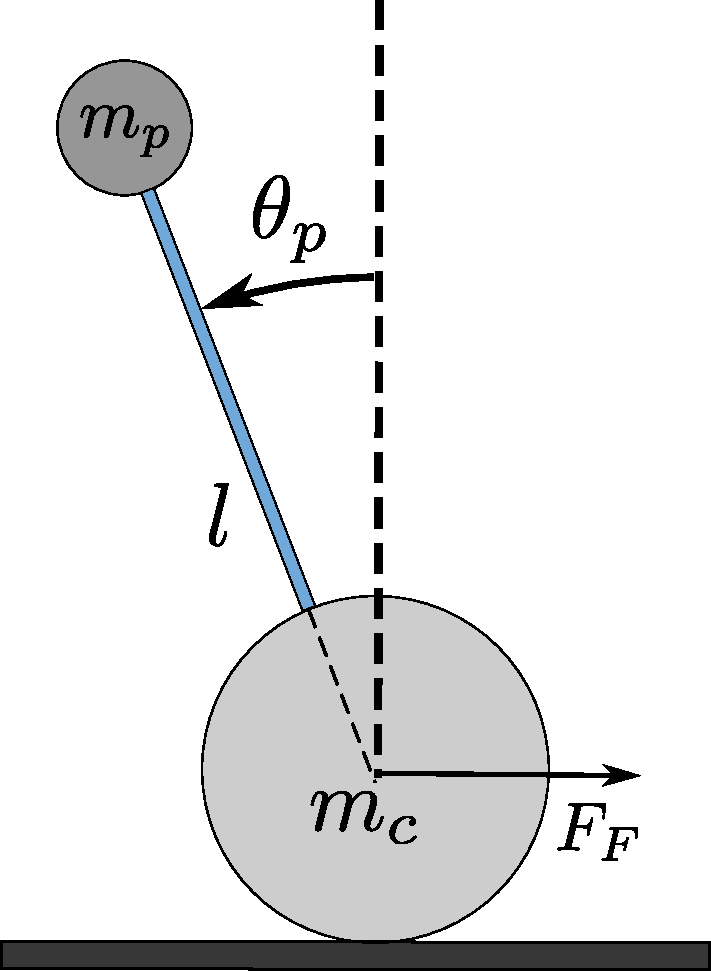
\includegraphics[width=0.25\textwidth]{/invertedPendulumModel.pdf}
\caption{An overall diagram of the segway.}
\label{fig:invertedPendulumModel}
\end{figure}
\vspace{-2em}
A figure of the segway with the cart mass, $m_c$, and inverted pendulum mass, $m_p$, can be seen in \autoref{fig:invertedPendulumModel}. Here, the inverted pendulum's tilting angle is represented by $\theta_p$, it can be further noted that the wheel's angle is denoted $\theta_w$.\\
The model of the segway is split in two smaller models, which is a model for the motor and wheel, and a model for the cart and inverted pendulum. These two models are later combined into a model for the segway. The splitting of the model can be seen in \autoref{fig:modelOverall}, together with the interfaces between the models.
\begin{figure}[H]
\centering
\input{figures/overallModel.rasmus}
\caption{The plant in the feedback loop. Within it is a motor and wheel model and a model for the inverted pendulum.}
\label{fig:modelOverall}
\end{figure}
\vspace{-2em}
The input to the system is the voltage applied to the motors, $V_a$. This voltage is controlled by simply changing the PWM duty cycle that controls the motors. In practice, this is equal to changing the motor input voltage. The interface signal between the motor and wheel model and the model describing the cart's movement is the torque applied by the motors to the cart, $\tau_a(t)$. Based on this torque, an expression for the force $F_F(t)$ can be made, which is the force that makes the segway move either forward or backwards.
The interface between the cart and the inverted pendulum is chosen to be the the angle of the wheels, $\theta_w$, as they determine the position of the segway. %This is the applied force to the segway, that makes it move. 
%The applied force, $F_F$,  is generated by the motors and wheels, and is what makes the segway move.\\
The model of the inverted pendulum has this angle, $\theta_w$ as input and the angle of the inverted pendulum, $\theta_p$, as output. Also, a load force $F_L(t)$ is inserted from the inverted pendulum to the cart model, as the tilting of the pendulum makes the cart move. % From the wheel angle, $\theta_w$, it is possible to set up an expression for the force that the wheels apply to the segway, named $F_F$, as this is used in the segway model.
%The reason why $F_F$ is chosen as the interface between the two smaller models is because it is usually such an input force that is used when modelling an inverted pendulum, see e.g. \citep{InvertedPendulumMathworks}. It will therefore be easy to put up a free body diagram of the inverted pendulum, since the contribution from the base to the pendulum is a force, easily included in the diagram.
\\\\
In this chapter, an expression for the motor and wheel model will be derived. Afterwards, a model of the cart and inverted pendulum is derived, see \autoref{fig:modelOverall}. These models will be simulated and verified, before being combined. Lastly the system model is simulated and verified. To be able to design a controller for the system, this model is then linearised and Laplace transformed to allow a transfer function to be derived, which is the final step performed in this chapter. %The transfer function of the system is the output of this chapter. \\
Firstly the motors and wheels model is to be derived in the following section. 
% From the model of the motors and wheels, a transfer function can be derived for the system. This transfer function can be be combined with a transfer function for the inverted pendulum, resulting in a transfer function for the entire plant.
%Thus the model transfer function can be described as a product of the partial system transfer functions:
%\begin{equation}
%G(s) = \frac{\theta_p(s)}{V_a(s)} = \frac{F_F(s)}{V_a(s)} \cdot \frac{\theta_p(s)}{F_F(s)}
%\label{eq:Gs_segway}
%\end{equation}
%
%\begin{where}
%\va{$G(s)$}{is the plant transfer function}{rad/V}
%\va{$V_a(s)$}{is the input voltage}{V}
%\va{$F_F(s)$}{is forward force}{N}
%\va{$\theta_p(s)$}{is the pendulum tilting angle}{rad}
%\end{where}
%\newpar
%Now that the model has been split up into two, each model will be separately derived. This is done in the following sections, starting with the motors and wheels model.
%The first step to create a control system for the segway is to model all the electrical and mechanical parts of the segway. The model determines how the segway behaves and can help to predict how it will react when a force or input is applied to different parts. The modelling of the segway is divided into two sections:% as seen on \autoref{fig:modelling_overview}.

%\begin{itemize}
%\item Modelling of the motors and wheels.
%\item Modelling of the inverted pendulum.
%\end{itemize}

%\begin{figure}[H]
%	\centering
%	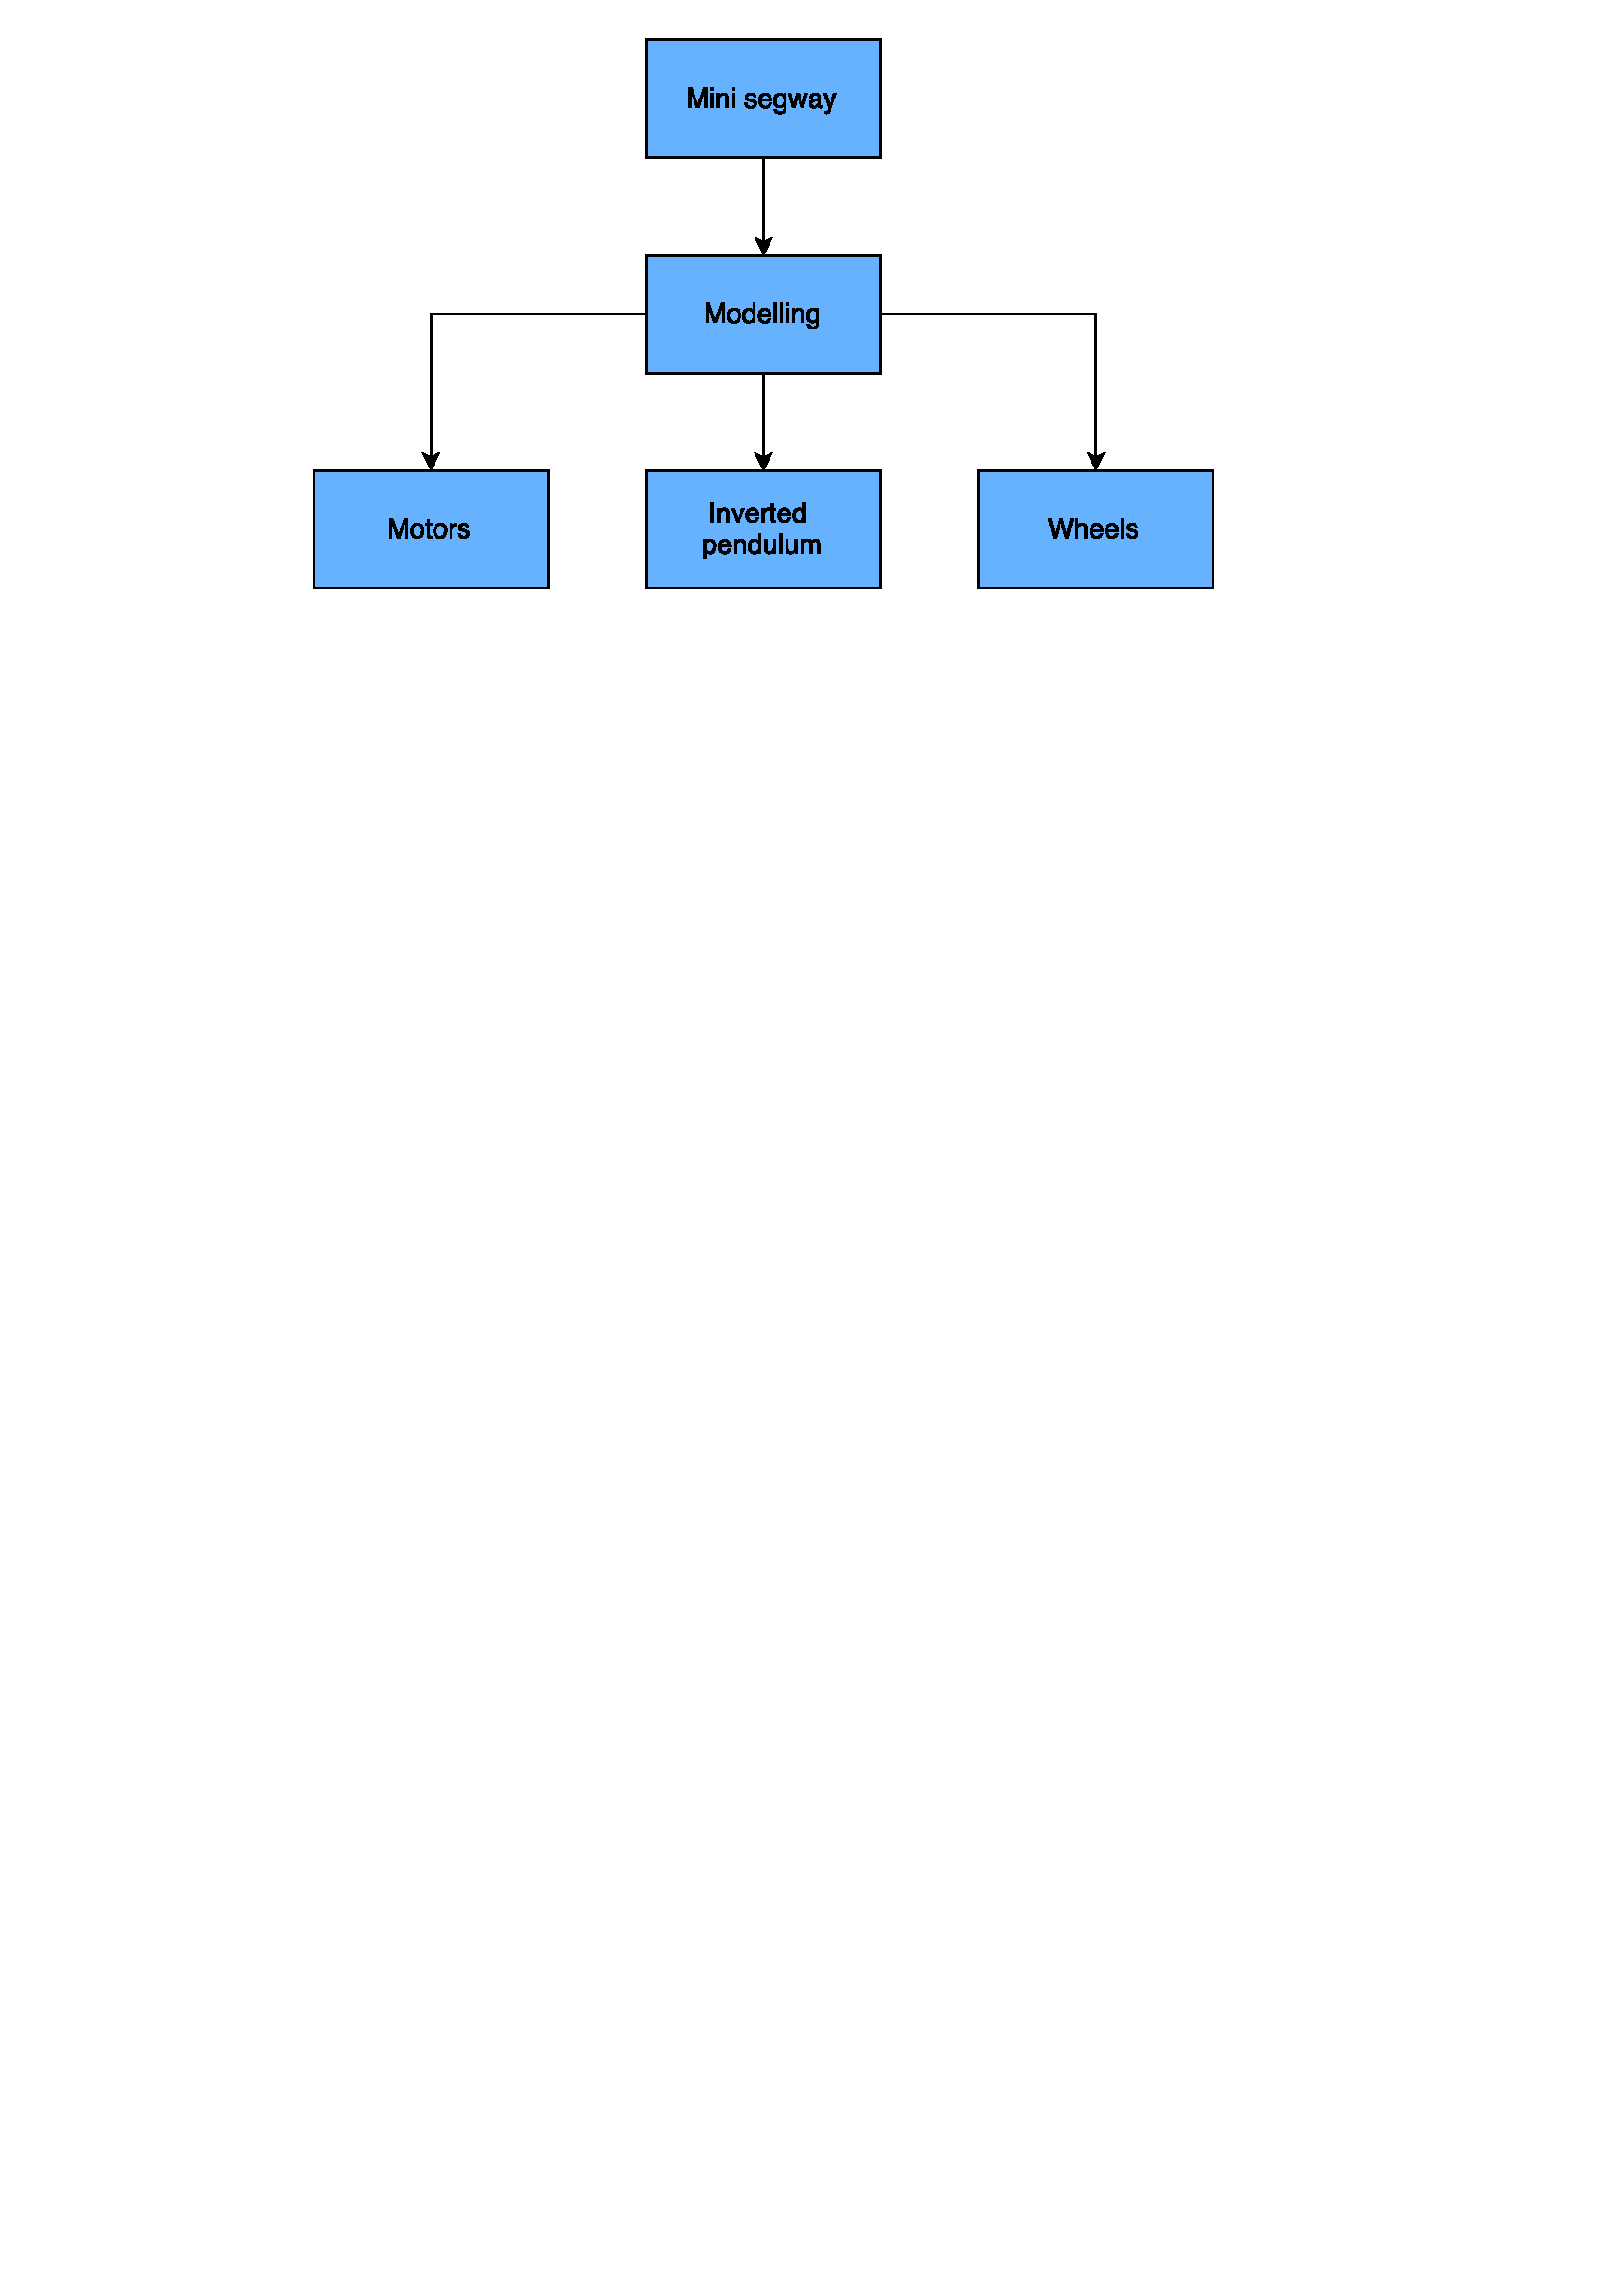
\includegraphics[width=0.7\textwidth]{design/figures/modelling/modelling_intro_block.pdf}
%	\caption{The division of the modelling.}
%	\label{fig:modelling_overview}
%\end{figure}

%The two sections are modelling of the inverted pendulum and modelling of the motors and wheels. The first part will consist of a modelling of the motors and wheels and the second part is the inverted pendulum. 

\section{Model of Motor and Wheel}
%An overall block diagram of the model of the motor and wheels can be seen on \autoref{fig:motorOverall}.
The model of the motors and wheels can be split into two parts; an electrical part and a mechanical part, since the two parts can be analyzed separately, though they are connected. This is due to the feedback that is present between the rotational velocity and the voltage, when modelling a motor \citep[15]{modelnote}.\\
The electrical model gives an output describing the motor current, $I_a(t)$. This is linked to the motor torque through the motor constant, $k_t$ \citep[p. 14]{modelnote}.\\
The mechanical part of the motor model describes both the motors, gears and wheels, since these are all connected. The mechanical part of the model has the angular velocity of the wheel, $\omega_w$ as output.
%A wheel model is also included to give the output of the motors and wheels model, that is the force applied, $F_F$, to the system by the motors and wheels.
A feedback is present in the system from $\omega_w$ to the applied voltage $v_a$, due to the back-EMF in the motor.\\
%\begin{figure}[H]
%\centering
%\scalebox{0.9}{
%\input{figures/overallMotor.rasmus}
%}
%\caption{An overall system diagram of the motor, gears and wheels.}
%\label{fig:motorOverall}
%\end{figure}
In the following, the electrical motor model is derived. Then, a mechanical model of the motors and wheels is put up. These two models can then be combined.\\
%\textbf{As the final step in the model of the motors and wheels, an expression for the applied force, $F_F$ is made, which can then be merged with the motor-wheel transfer function.}\\
Note that the modelling will be based on a single motor and wheel system, as the two motors and wheels on the segway are assumed identical. However, when deriving the expression for the applied force, $F_F$, both motors and wheels in the system are accounted for.
%After this, the inverted pendulum is modelled. This model can be combined with the motors and wheels model, to get the transfer function for the entire plant, as described in \autoref{fig:modelOverall}.\\
%In the following section, the electrical part of the motor is modelled.
\subsection{Electrical Motor Model}
The electrical part of a motor can be modelled using a resistor, $R_a$, an inductor, $L_a$, and a voltage generator, $V_e$, which delivers a voltage proportional to the motor's angular velocity $\omega_m$, also known as the back-EMF voltage \citep[p. 15]{modelnote}. This can be seen in \autoref{fig:motor_electrical}, where the input voltage, $V_a$, and the motor current, $I_a$, are shown, with the index $a$ denoting the armature of the motor. This model assumes that it is a permanent magnet DC motor that is used \citep[p. 15]{modelnote}, but as explained in section \ref{subsec:motors}, the motors used are of this type, meaning the model structure is valid.
\begin{figure}[H]
\centering
\begin{circuitikz}[american voltages]

	% electrical equivalent circuit
	\draw (0,0) to[V, v^=$V_a$] (0,3);
	\draw (0,3) to[R, i>^=$I_a$, l=$R_a$] (3,3);
	\draw (3,3) to[L, l=$L_a$] (4,3);

	\draw (4,3) -- (5,3);
	\draw (5,0) to[V, v_=\mbox{$V_e = k_e\omega_m$}] (5,3);
	\draw (0,0) -- (5,0);

\end{circuitikz}
\caption{Electrical curcuit equivalent of a DC motor.}
\label{fig:motor_electrical}
\end{figure}
Kirchoff's voltage law is applied to the circuit yielding the following expression:
\begin{equation}
0 = V_a(t) - R_a\cdot I_a(t) - L_a \dot{I_a}(t) - V_e(t) \label{eq:kirchoffsV}
\end{equation} 
\begin{where}
\va{$V_a(t)$}{is the motor input voltage}{V}
\va{$R_a$}{is the motor resistance}{$\Omega$}
\va{$L_a$}{is motor inductance}{H}
\va{$I_a(t)$}{is motor current}{A}
\va{$V_e(t)$}{is the back-EMF}{V}
\end{where}

%The equation is Laplace transformed to give the following:
%\begin{equation}
%\label{eq:electricMotor}
%0 = V_a(s) - R_a\cdot I_a(s) - s L_a I_a(s) - V_e(s)
%\end{equaeetion}

%$V_e$ is proportional to the motor velocity \citep[p. 15]{modelnote}, i.e.:
\clearpage
The back-EMF is directly proportional to the rotational speed of the motor:
\begin{equation}
V_e(t) = k_e \cdot\omega_m(t)
\end{equation}
\begin{where}
\va{$\omega_m(t)$}{is the rotational speed of the motor}{$\text{rad}/$s}
\va{$k_e$}{is the back-EMF constant}{V$/{\frac{\text{rad}}{s}}$}
\end{where}

Now, the expression for $V_e(t)$ can be inserted in \autoref{eq:kirchoffsV}. The equation is isolated for $I_a(t)$, since the current is the interface between the electrical and mechanical parts of the model. It is assumed that $\dot I_a(t) = 0$, since the electrical time constant is usually much higher than mechanical time constant \citep[p. 74]{sou:Feedback}. This yields \autoref{eq:electricMotor2}.
\begin{equation}
\label{eq:electricMotor2}
I_a(t) = \frac{1}{R_a} \left( V_a(t) - k_e \cdot \omega_m(t) \right)
\end{equation}
The torque of a motor is proportional to the current \citep[p. 14]{modelnote}:
\begin{equation}
\tau_m(t) = k_t \cdot I_a(t)
\label{eq:currenttau11}
\end{equation}
\begin{where}
\va{$\tau_m(t)$}{is the torque of the motor}{Nm}\\
\va{$k_t$}{is the motor constant}{Nm/A}\\
\end{where}

Inserting the expression for the current $I_a(t)$ from \autoref{eq:electricMotor2} into \autoref{eq:currenttau11} gives the following:
\begin{equation}
\label{eq:voltageToTorque}
\tau_m(t) = \frac{k_t}{R_a} \left( V_a(t) - k_e \omega_m(t) \right)
\end{equation}
%
%A block diagram of \autoref{eq:voltageToTorque} can be put up, see \autoref{fig:motorGearBlock}. Here, the input is the applied voltage $V_a(t)$, and the output the motor angular velocity, $\omega_m(t)$.
%
%Notice that a block describing the mechanical motor-wheel system has been inserted to transfer from torque, $t_m(t)$ to the angular velocity of the motor, $\omega_m(t)$. 
%%A gear transfer function is also inserted, to obtain the angular velocity of the wheel, $\omega_w(s)$ from the motor angular velocity, $\omega_m(s)$.
%
%\begin{figure}[H]
%\centering
%\input{figures/electricalMotor.rasmus}
%\caption{A block diagram of the motor and gearing.}
%\label{fig:motorGearBlock}
%\end{figure}

A model for the gears and wheel needs to be determined to find the torque $\tau_a$ that is applied to the segway, since the inertias and dampers in the gear-wheel setup influences this. This is done in the following section.
%In the next section, the transfer function for the mechanical system and the gears, describing the relationship between motor torque $\tau_m(s)$ and the rotational speed of the motor, $\omega_m(s)$, as well as the relationship between $\omega_m(s)$ and $\omega_w(s)$.

%In the feedback on \autoref{fig:motorGearBlock}, a transfer function describing the gearing is also needed, to describe the motor angular velocity $\omega_m(s)$ based on the wheel angular velocity, $\omega_w(s)$. These two gear transfer functions are derived in the following section. 
%To transfer from $\omega_w$ to $\omega_m$, the inverted gear ratio is inserted, since this is the connection between the two angular velocities.

%Ideally, the function in \autoref{eq:voltageToTorque} is turned into a transfer function describing the relationship between input voltage and motor torque. This is however not possible, since the gearing transfer functions are not yet known. Thus, these need to be determined before the transfer function for the system can be put up. 
%In the next section, the transfer function for the gears, describing the relationship between motor torque $\tau_m(s)$ and the rotational speed of the outer wheel, $\omega_w(s)$ can found. 
\subsection{Mechanical Motor and Wheel Model}
%The transfer function from motor torque $\tau_m$, to the angular velocity of the motor, $\omega_m$, is now to be found.
A model for the mechanical behaviour of the motors and wheels is to be found, so it can be combined with the electrical model for the motors, thus forming the combined model for the motors and wheels. \\
It is necessary to take the entire mechanical system, eg. both wheels and gearing ratios, into account, as these affect the motor's rotation.

\subsubsection{Gear relations}
First, the configuration of the gears are determined before the modelling can begin. The motor and wheel system consists of a DC motor, which has a gear mounted. The output of this gear is applied to the motor shaft, onto which a secondary gear is mounted. The inner wheel gear is mounted directly on the shaft, and thus has the same angular velocity as the motor. Therefore their inertia can be seen as one, being the shaft inertia. The configuration of the gears can be seen in \autoref{fig:gears}.
\begin{figure}[H]
\centering
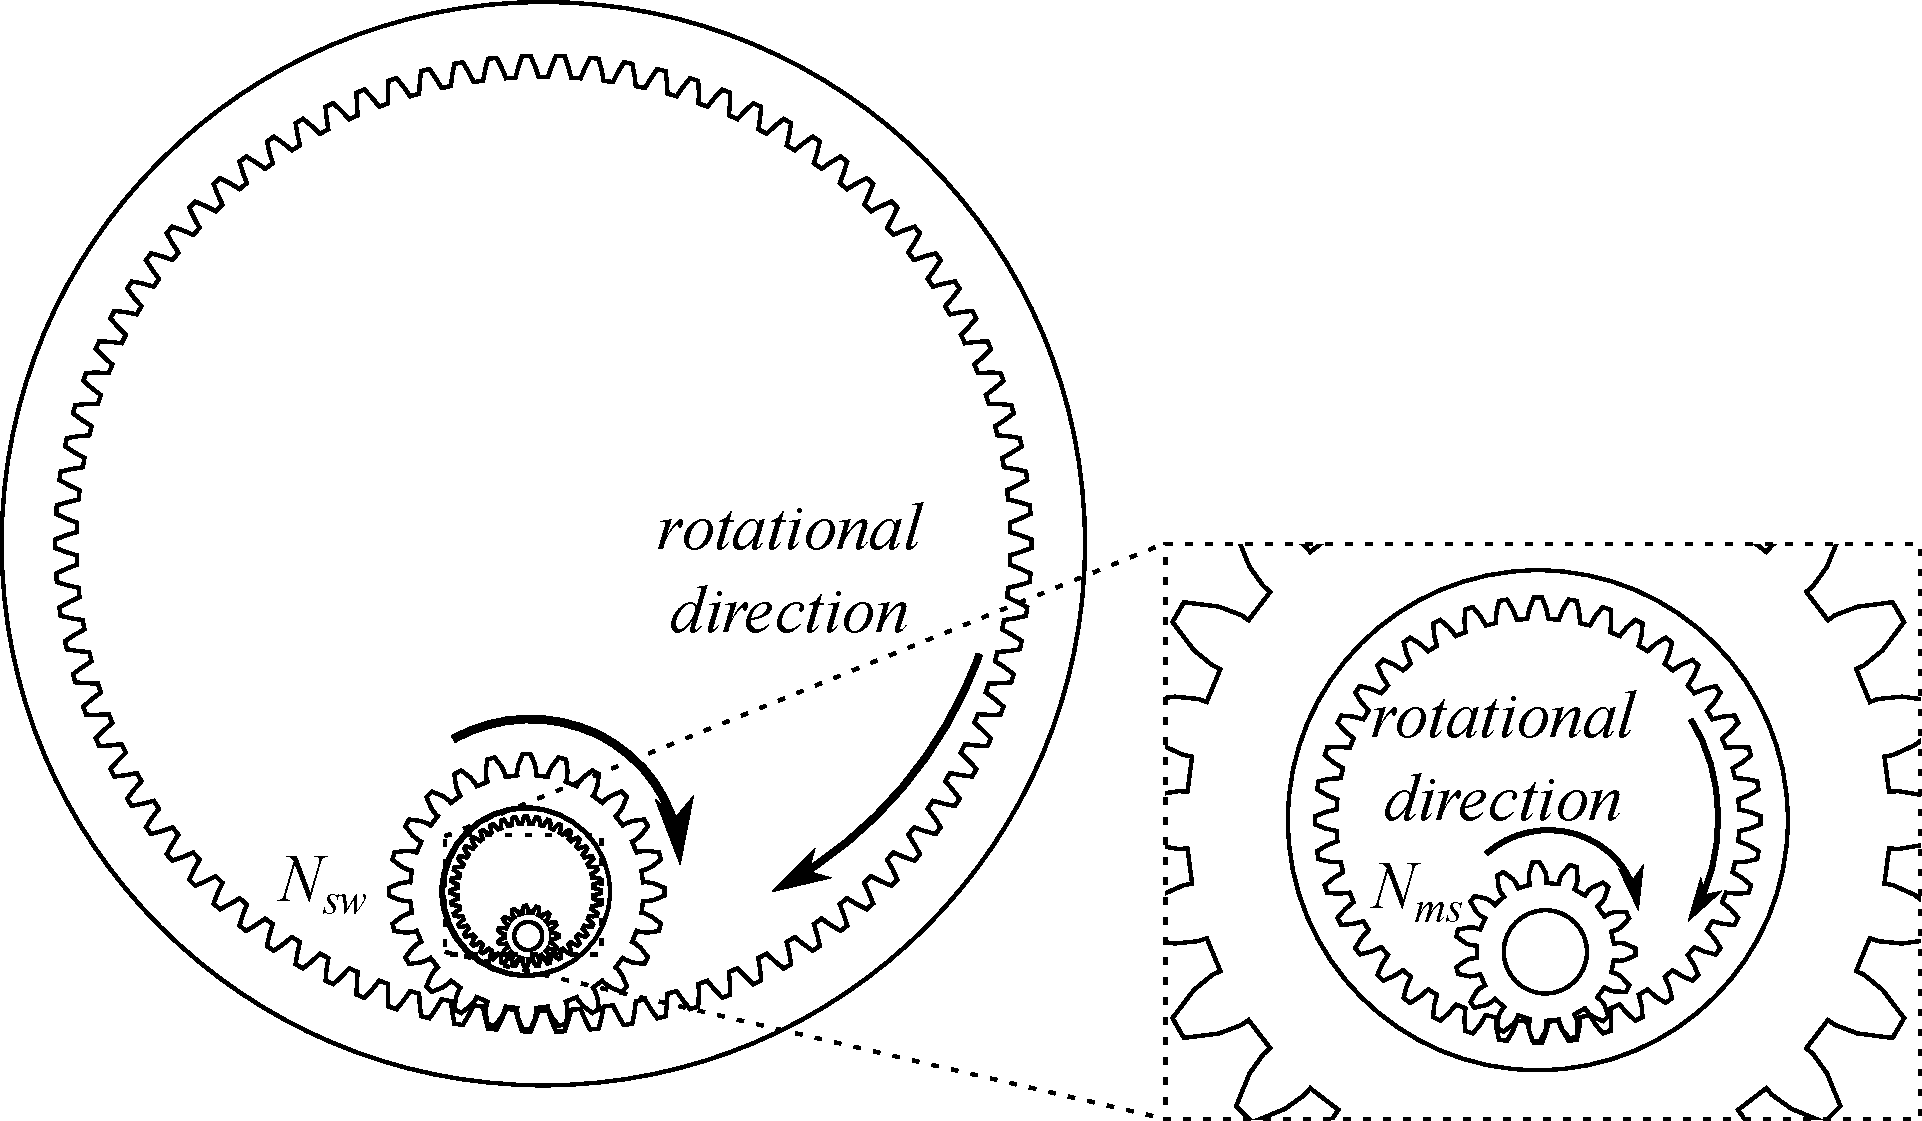
\includegraphics[width=0.75\textwidth]{figures/gears.pdf}
\caption{The different parts of the wheel's rotational system and its relative direction of rotation along with the gear ratios, $N_{ms}$ and $N_{sw}$.}
\label{fig:gears}
\end{figure}
In \autoref{fig:gears} the gear ratio between the motor and shaft is shown as $N_{ms}$, and the gear ratio for the shaft and wheel as $N_{sw}$.
\begin{figure}[H]
\centering
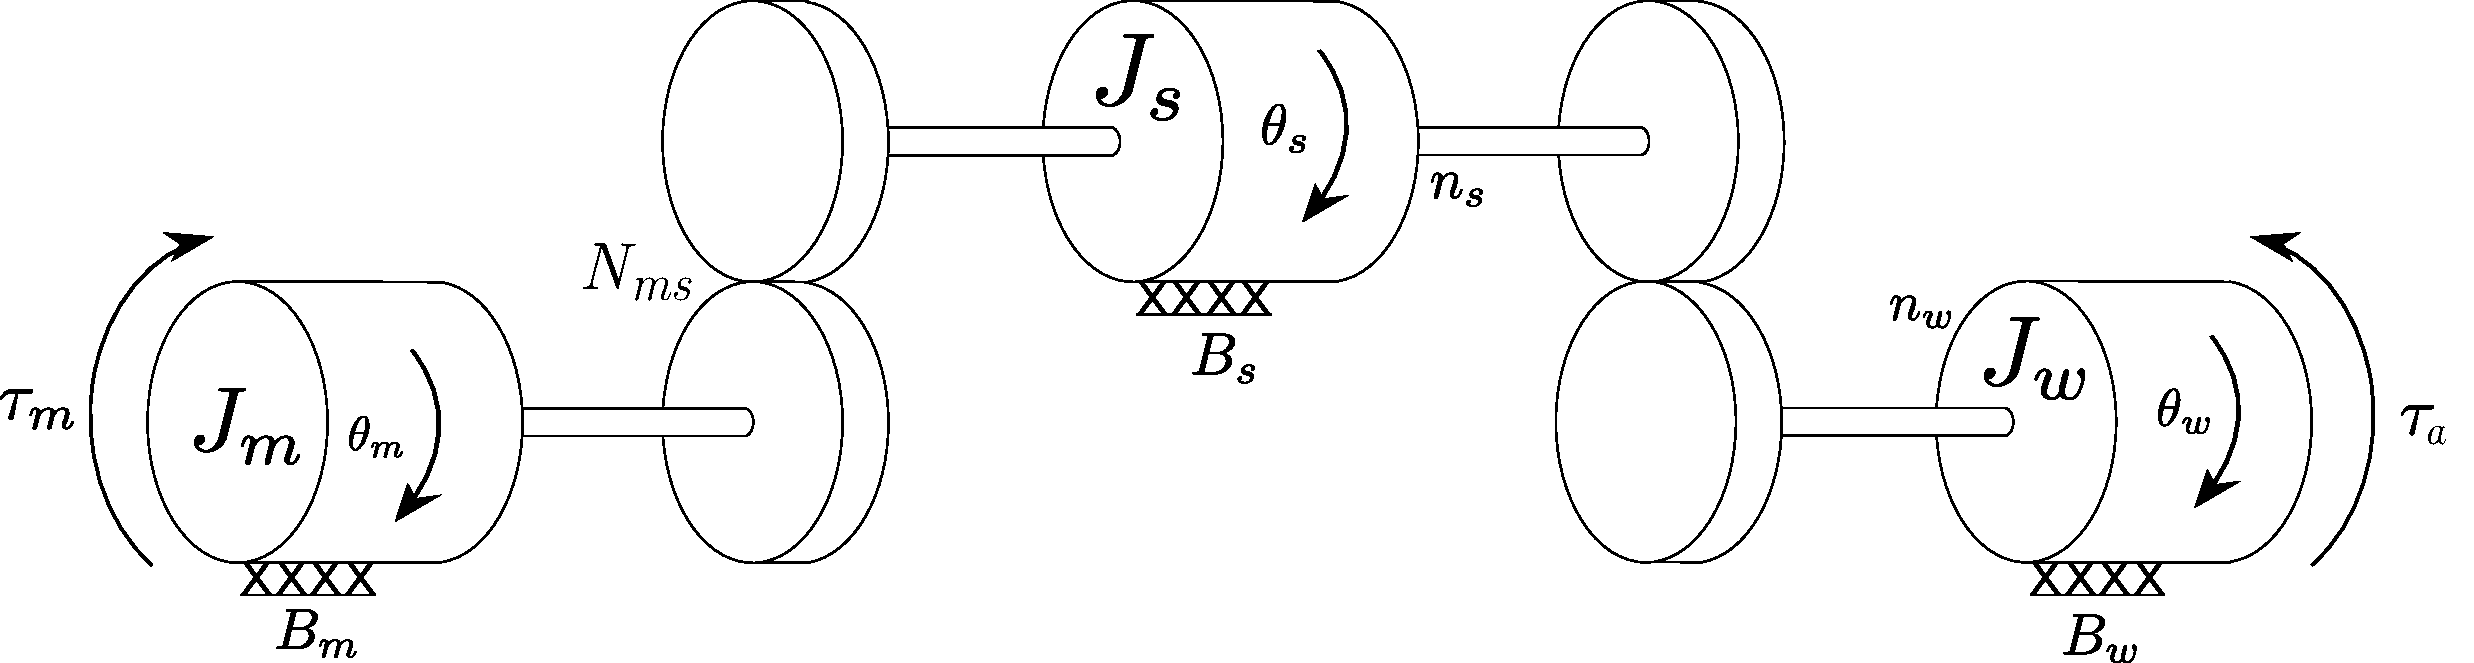
\includegraphics[width=\textwidth]{figures/motorRotationalDiagram.pdf}
\caption{Mechanical model of the motor and wheel setup.}
\label{fig:motorRotational}
\end{figure}

The gear ratio is used to determine the relation between angle and its derivatives for two or more rotational objects. The basis for determining is \autoref{fig:gearsRelation}, where it is assumed that there is no sliding between two gears. A torque $\tau_1$ is applied to the inner gear, giving it a certain angular position, $\theta_1$. The second gear also has a torque, $\tau_2$ and an angular position, $\tau_2$. Since the two gears have to move the same amount when rotating, as no slipping is assumed, \autoref{eq:gearRatio} can be put up, from which the gear ratio can be determined.

\begin{figure}[H]
\centering
\scalebox{1}{\input{figures/MotorAndWheel.ralf}}
\caption{Correlation of gears.}
\label{fig:gearsRelation}
\end{figure}

\begin{equation}
\theta_1r_1 = \theta_2r_2 \Rightarrow N = \frac{r_1}{r_2} = \frac{\theta_2}{\theta_1} = \frac{\omega_2}{\omega_1}
\label{eq:gearRatio}
\end{equation}
\begin{where}
\va{$N$}{The gear ratio}{1}
\va{$\theta_1$}{Angle of the inner gear}{rad}
\va{$\theta_2$}{Angle of the outer gear}{rad}
\va{$r_1$}{The radius of the inner gear}{m}
\va{$r_2$}{The radius of the outer gear}{m}
\va{$\omega_1$}{Angle velocity of the inner gear}{rad/s}
\va{$\omega_2$}{Angle velocity of the outer gear}{rad/s}
\end{where}

This, however, does not yield the relation between the torque of the gears and the gear ratio. This relation can be obtained through steady state analysis of each gear. This yields \autoref{eq:steadyGear1} and \autoref{eq:steadyGear2} for the inner and outer gear respectively, since the force of the two gears are of the same magnitude, i.e. $F_{g1}$ = $F_{g2}$ = $F_g$. This is because the force one gear excerts on the other is balanced by an equal, but opposite force, in correlation with Newton's 3rd law of motion. Based on this, it is possible to put up the following equations:
\begin{align}
\tau_1 - r_1\cdot F_g = 0 \label{eq:steadyGear1}
\\
\tau_2 - r_2\cdot F_g = 0\label{eq:steadyGear2}
\end{align}
\begin{where}
\va{$F_g$}{Translatoric force that works against the gear.}{N}
\end{where}

Thus, the gear ratio affects the relation between the torque in the two gears as shown in \autoref{eq:torqueRelation}.
\begin{equation}
\frac{\tau_1}{\tau_2} = \frac{r_1}{r_2} = N
\label{eq:torqueRelation}
\end{equation}

To describe the relation of the torque and the angle for two or more gears, the gear ratio, N, must be determined. This is done through the number of cogs in each cogwheel, as this can be thought of being equivalent to the wheel radii, which has previously been used to determine the gear ratio. From \autoref{subsec:wheels}, it's known that $n_s = 25$ and $n_w = 90$. From these, the gear ratio can be found.

\begin{equation}	
N_{sw} = \frac{n_s}{n_w} = \frac{\theta_w(t)}{\theta_s(t)} = \frac{25}{90} \approx 0.2778
\label{Nsw}
\end{equation}
\begin{where}
\va{$N_{sw}$}{is the shaft-wheel gear ratio}{1}\\
\va{$n_s$}{is number of cogs on the motor gear}{1}\\
\va{$n_w$}{is number of cogs on the wheel}{1}\\
\va{$\theta_s(t)$}{is the motor angle}{rad}\\
\va{$\theta_w(t)$}{is the wheel angle}{rad}\\
\end{where}

From \citep{gear} the gear ratio from motor to shaft is known:
\begin{equation}
N_{ms} = \frac{1}{19} \approx 0.053
\label{Nms}
\end{equation}
With the gear relations determined, it is now possible to derive the mechanical motor and wheel model.
\vspace{0.4 cm}
\subsubsection{Derivation of Mechanical Motor and Wheel Model}
\vspace{0.3 cm}
Now that the configuration of the rotational system is known, the motor, shaft and wheel system can be drawn using ideal elements, i.e. inertias and dampers, which can be seen in \autoref{fig:motorRotational}. Note, that all gears are assumed to have an inertia and a friction as no gears are assumed ideal. Also note that the friction in the gears is modelled as a damper, and thus each of the friction torques can be described in the same way as the friction torque for the shaft shown here: $\tau_{B_s}(t) = B_s \cdot \omega_s(t)$. The coulomb friction which is also present is not taken into account, due to the fact that an offset in the software can take care of this non-linearity, which is not easily modelled.\\
\clearpage
In \autoref{fig:motorRotational} it is seen how the motor connects to the shaft, which again connects to the wheel. All connections are made through gears. The constants $n_s$ and $n_w$, are the number of cogs on the shaft and wheel cog-wheels. These are used to determine the gear ratios.\newpar
The input torque to the motor $\tau_m(t)$, see \autoref{fig:motorRotational}, sets the direction of all the resultant angular positions, and therefore also angular velocities and angular accelerations in accordance with \autoref{fig:gears}.\\
The free body diagrams of the motor, shaft and wheel are illustrated in \autoref{fig:FBDMotorShaftWheel}. %In the motor part \autoref{fig:FBDMotor}, the motor torque, $\tau_m$, is inserted along with a friction torque, $\tau_{B_m}$, and a gearing torque transferring torque to the wheel.
%In the wheel part \autoref{fig:FBDWheel}, the gear torque, $\tau_{G_w}$, is inserted, along with a friction torque. The resultant torques are also shown.
\begin{figure}[H]
\centering
\begin{subfigure}[b]{0.3\textwidth}		
        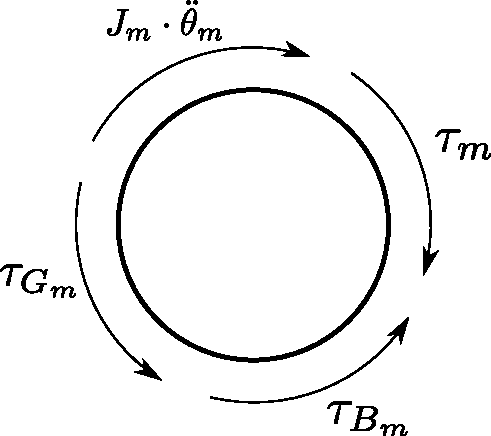
\includegraphics[width=0.98\textwidth]{figures/FBD/FBDMotor.pdf}
        \vspace{3.5mm}
        \caption{FBD of rotational system for the motor.}
        \label{fig:FBDMotor}
    \end{subfigure} 
    \hspace{4mm} 
\begin{subfigure}[b]{0.3\textwidth}
        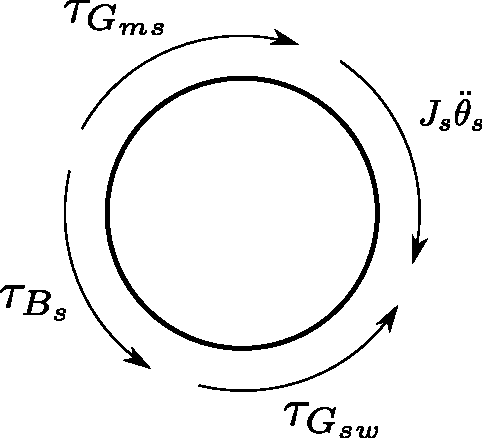
\includegraphics[width=0.95\textwidth]{figures/FBD/FBDShaft.pdf}
        \vspace{2mm}
        \caption{FBD of rotational system for the shaft.}
        \label{fig:FBDshaft}
    \end{subfigure}  
    \hspace{4mm} 
\begin{subfigure}[b]{0.3\textwidth}
        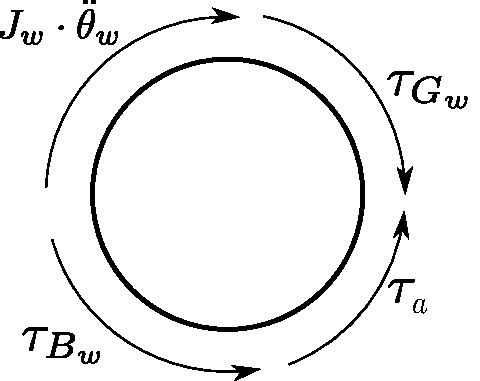
\includegraphics[width=0.95\textwidth]{figures/FBD/FBDWheel.pdf}
        \vspace{5mm}
        \caption{FBD of rotational system for the wheel.}
        \label{fig:FBDWheel}
    \end{subfigure}
\caption{Free body diagrams of the three rotational systems.}
\label{fig:FBDMotorShaftWheel}
\end{figure}
Note that the following relationships between the gear torques exist, based on the gear ratios: 
\begin{equation}
\tau_{G_{ms}}(t) = \tau_{G_m}(t) \cdot \frac{1}{N_{ms}}
\label{gearTorqueMotor}
\end{equation}
\begin{equation}
\tau_{G_w}(t) = \tau_{G_{sw}}(t) \cdot \frac{1}{N_{sw}}
\label{gearTorqueWheel}
\end{equation}
\begin{where}
\va{$\tau_{G_{ms}}(t)$}{is the torque from motor to shaft}{Nm}\\
\va{$\tau_{G_m}(t)$}{is the torque to shaft from motor}{Nm}\\
\va{$\tau_{G_w}(t)$}{is the torque from shaft to wheel}{Nm}\\
\va{$\tau_{G_{sw}}(t)$}{is the torque to wheel from shaft}{Nm}\\
\end{where}

From \autoref{fig:FBDMotorShaftWheel}, the following differential equations can be put up:
\begin{align}
J_m\ddot\theta_m(t) &= \tau_m(t) -\tau_{G_m}(t) - \tau_{B_m}(t)\label{eq:DE1}\\
J_s\ddot\theta_s(t) &= \tau_{G_{ms}}(t) - \tau_{G_{sw}}(t) - \tau_{B_s}(t)\label{eq:DE2}\\
J_w\ddot\theta_w(t) &= \tau_{G_{w}}(t) - \tau_{B_w}(t) -\tau_a(t) \label{eq:DE3}
\end{align}

\begin{where}
\va{$J_m$}{is the motor moment of inertia}{$\text{kg} \cdot \text{m}^2$}\\
\va{$J_s$}{is the shaft moment of inertia}{$\text{kg} \cdot \text{m}^2$}
\va{$J_w$}{is the wheel moment of inertia}{$\text{kg} \cdot \text{m}^2$}
\va{$\ddot\theta_m(t)$}{is the angular acceleration of the motor}{$\text{rad}/\text{s}^2$}\\
\va{$\ddot\theta_s(t)$}{is the angular acceleration of the shaft}{$\text{rad}/\text{s}^2$}\\
\va{$\ddot\theta_w(t)$}{is the angular acceleration of the wheel}{$\text{rad}/\text{s}^2$}\\
\va{$\tau_m(t)$}{is the delivered torque from the motor}{$\text{rad}/\text{s}^2$}\\
\va{$\tau_{B_m}(t)$}{is the motor friction torque}{Nm}\\
\va{$\tau_{B_s}(t)$}{is the shaft friction torque}{Nm}\\
\va{$\tau_{B_w}(t)$}{is the wheel friction torque}{Nm}\\
\va{$\tau_{a}(t)$}{is the torque applied to the cart}{Nm}\\
\end{where}

In the following, a model for the motors and wheels system is obtained. This is done using the differential equations derived from the free body diagrams, see \autoref{eq:DE1}, \autoref{eq:DE2} and \autoref{eq:DE3}.
%\textbf{In the following, a transfer function for the gearing/wheel system is obtained. The input to the system is the motor torque, $\tau_m(t)$, and the output is the angular velocity of the wheel, $\omega_w(t)$.
%This is done using the differential equations derived from the free body diagrams, see \autoref{eq:DE1}, \autoref{eq:DE2} and \autoref{eq:DE3}. It is desired to combine these equations, to obtain a transfer function for the entire mechanical model.\todo{not looking for a transferfunction. Rewrite}}
\\The model is derived by working from the outside and in, starting with the equations for the wheel and inserting them to get an expression for the motor that includes the wheel and shaft.\\
The differential equation for the wheel rotational system, \autoref{eq:DE3}, states:
\begin{equation}
J_w\ddot\theta_w(t) = \tau_{G_{w}}(t) - \tau_{B_w}(t) - \tau_a(t) \nonumber
\end{equation}
The linear approximation of the friction torque, which is modelled as a damper, can be described as $\tau_{B_s}(t) = B_s \cdot \dot\theta_s(t)$. Inserting this together with the expression for the gear torque from \autoref{gearTorqueWheel} gives:
\begin{equation}
J_w \ddot\theta_s(t) N_{sw} = \tau_{G_{sw}}(t)\cdot \frac{1}{N_{sw}} - {B_{w}} N_{sw} \cdot \dot\theta_{s}(t) -\tau_{a}(t)
\end{equation}
%Laplace transforming the equation and isolating for $\tau_{G_{sw}}$ gives:
%\begin{equation}
%s^2 J_w N_{sw} \theta_s(s) = \tau_{G_{sw}}(s)\cdot \frac{1}{N_{sw}} - s {B_{w}} N_{sw} \cdot \theta_{s}(s)
%\end{equation}
%\begin{equation}
%\tau_{G_{sw}}(s) = \theta_s(s) \cdot N_{sw}^2 (s^2 J_w + s B_w) 
%\label{tauGSW}
%\end{equation}
Isolating for $\tau_{G_{sw}}$ gives:
\begin{equation}
\tau_{G_{sw}}(t) = J_w \ddot\theta_s(t) N_{sw}^2 + B_wN_{sw}^2\dot\theta_s(t) + \tau_a(t) \cdot N_{sw}
\label{tauGSW}
\end{equation}
Now that an expression for $\tau_{G_{sw}}(t)$ is obtained, it can be combined with the differential equation for the second rotational system, \autoref{eq:DE3}, which states:
\begin{equation}
J_s\ddot\theta_s(t) = \tau_{G_{ms}}(t) - \tau_{G_{sw}}(t) - \tau_{B_s}(t) \nonumber
\end{equation}
The friction can, as previously mention be described as $\tau_{B_s}(t) = B_s \cdot \dot\theta_s(t)$. Inserting this and isolating for $\tau_{G_{ms}}(t)$ yields:
\begin{equation}
\tau_{G_{ms}}(t) = \tau_{G_{sw}}(t) + B_s \cdot \dot\theta_s(t) + J_s\ddot\theta_s(t) 
\label{tauGSAlmost}
\end{equation}
\autoref{tauGSW} is inserted in \autoref{tauGSAlmost} together with the expression for the motor-shaft gear from \autoref{gearTorqueMotor}. An expression for $\tau_{G_m}(t)$ can thus be found:
%\begin{equation}
%\tau_{G_{ms}}(t) = \left(J_w \ddot\theta_s(t) N_{sw}^2 + B_wN_{sw}^2\dot\theta_s(t) + \tau_a(t)\right) + B_s \cdot \dot\theta_s(t) + J_s\ddot\theta_s(t) 
%\label{tauGS}
%\end{equation}
%Inserting the motor-shaft gear ratio, an expression for $\tau_{G_m}(t)$ can be obtained:
%\begin{equation}
%\tau_{G_{m}}(s)\frac{1}{N_{ms}} = \theta_m(s){N_{ms}}(s^2(J_s + N_{sw}^2 J_w) + s (B_s + N_{sw}^2 B_w))\label{tauGMAlmost}
%\end{equation}
\begin{equation}
\tau_{G_{m}}(t) = J_w \ddot\theta_m(t) N_{ms}^2 N_{sw}^2 + B_w N_{ms}^2 N_{sw}^2\dot\theta_m(t) + \tau_a(t)\cdot N_{ms} N_{sw} + B_s N_{ms}^2 \cdot \dot\theta_m(t) + J_s N_{ms}^2 \ddot\theta_m(t) 
\label{tauGM}
\end{equation}

This expression can be combined with the differential equation for the motor rotational system, as seen in \autoref{eq:DE1} and stated here:
\begin{equation}
J_m\ddot\theta_m(t) = \tau_m(t) -\tau_{G_m}(t) - \tau_{B_m}(t) \nonumber
\end{equation}
Inserting the expression for the friction torque, $\tau_{B_m}(t) = B_m \cdot \dot\theta_m(t)$ and $\tau_{G_{m}}(t)$ as found in \autoref{tauGM} yields \autoref{eq:tauM(t)} where the motor torque $\tau_m(s)$ has also been isolated:\vspace{0.3 cm}
%\begin{equation}
%s^2 J_m \theta_m(s) = \tau_m(s) - \tau_{G_{m}}(s) - s{B_m}\theta_m(s)
%\end{equation}
%
%The motor torque, $\tau_m(s)$ is isolated:
\begin{align}
\begin{split}
\tau_m(t) = &J_m\ddot\theta_m(t) + B_m \cdot \dot\theta_m(t)+ ( J_w \ddot\theta_m(t) N_{ms}^2 N_{sw}^2 + \\ & B_w N_{ms}^2 N_{sw}^2\dot\theta_m(t) + \tau_a(t)\cdot N_{ms} N_{sw} + B_s N_{ms}^2 \cdot \dot\theta_m(t) + J_s N_{ms}^2 \ddot\theta_m(t) )
\end{split}
\label{eq:tauM(t)}
\end{align}
This simplifies to:
\begin{align}
\begin{split}
\tau_m(t) = &\ddot\theta_m(t)\left(J_m + N_{ms}^2(J_s  + J_w N_{sw}^2) \right) + \dot\theta_m(t)\left(B_m + N_{ms}^2(B_s + N_{sw}^2 B_w)\right) + \tau_a(t)\cdot N_{ms} N_{sw}
\end{split}
\label{eq:tauM(t)2}
\end{align}
To simplify the expressions, the following definitions are made for the total equivalent inertia, $J_T$ and the total equivalent friction, $B_T$:
\begin{align}
J_{T} &\equiv J_m + N_{ms}^2(J_s + N_{sw}^2 J_w)\label{TotalInertia}\\
B_{T} &\equiv B_m + N_{ms}^2(B_s + N_{sw}^2 B_w)\label{TotalDamper}
\end{align}

This means that the expression can be written as:
\begin{align}
\begin{split}
\tau_m(t) = &\ddot\theta_m(t)\cdot J_T + \dot\theta_m(t) \cdot B_T + \tau_a(t)\cdot N_{ms} N_{sw}
\end{split}
\label{eq:tauM(t)3}
\end{align}
Using this and inserting the motor torque, \autoref{eq:voltageToTorque}, and isolating for $\tau_a(t)$ yields:
\begin{equation}
\tau_a(t) = \frac{1}{N_{ms} N_{sw}}\left(\frac{k_t}{R_A} \left( V_a(t) - k_e \dot\theta_m(t) \right) - \ddot\theta_m(t)J_{T} - \dot\theta_m(t)B_{T}\right) 
\label{eq:MotorFinal}
\end{equation}
\autoref{eq:MotorFinal} is the final model expression for the motors and wheels part of the system. Now the model of the inverted pendulum is to be found. These model expressions are then to be combined. From this a controller can be designed and later implemented. The deriviation of the inverted pendulum model is done in the following section. 
%
%
%%
%%Using the gear ratios, an expression for the wheel position, $\theta_w(s)$ is obtained:
%%\begin{equation}
%%\tau_m(s) = \theta_w(s) \frac{s^2 (J_m + N_{ms}^2(J_s + N_{sw}^2 J_w)) + s (B_m + N_{ms}^2(B_s + N_{sw}^2 B_w)) }{N_{ms} N_{sw}}
%%\end{equation}
%
%\subsection{Combined motors and wheels model}
%In the following section, the electrical motor model is combined with the mechanical model, to derive an expression for the transfer function $\frac{F_F(s)}{V_a(s)}$.
%
%First, the an expression for the angular velocity of the wheel, $\omega_w$ needs to be derived, based on the angular velocity of the motor, $\omega_m$. This relationship is quite simple, as it is defined by the gear ratios, as can be seen in \autoref{Nsw}. Since there are two gears, the motor-shaft gear and the shaft-wheel gear, both of these gear ratios needs to be included. Thus, the transfer function for the two gears become:
%\begin{equation}
%\frac{\omega_w(s)}{\omega_m(s)} = N_{ms} N_{sw}
%\label{omegaTF}
%\end{equation}
%
%The translational force caused by a rotational system can be described as: 
%\begin{align*}
%F_F &= 2 m_w \cdot a_w \\
%&= 2 m_w\cdot r_w\alpha_w \\
%&= 2 m_w\cdot r_w \dot\omega_w
%\end{align*}
%\todo{maybe use mass of cart instead of wheel}
%\begin{where}
%\va{$F_F$}{is the resultant applied force of the wheels}{N}\\
%\va{$m_w$}{is the mass of the wheel}{kg}\\
%\va{$a_w$}{is translatoric acceleration of the wheel}{m/$\text{s}^2$}\\
%\va{$r_w$}{is the radius of the wheel}{m}\\
%\va{$\alpha_w$}{is angular acceleration of the wheel}{rad/$\text{s}^2$}\\
%\va{$\omega_w$}{is the angular velocity of the wheel}{rad/$\text{s}^2$}\\
%\end{where}
%
%The reason why a factor of 2 has been multiplied with the expression is because there are two wheels, each exerting their own applied force. The combined force is therefore the sum of these, which is the same as multiplying with two if the forces are assumed identical. 
%
%The transfer function from rotational speed of the wheel, $\omega_2$ to the force $F_F$ can thus be described as:
%\begin{equation}
%\frac{\F_F(s)}{\omega_w(s)} = 2 s r_w m_w
%\label{OmegaToForce} 
%\end{equation}
%
%It is now possible to combine the equations for the electrical system with the equations for the mechanical system:
%
%The transfer function $\frac{\omega_m(s)}{\tau_m(s)}$ can be inserted in \autoref{fig:motorGearBlock} in the mechanic system block. Also, the transfer functions $\frac{omega_w(s)}{\omega_m(s)}$ and $\frac{F_F(s)}{\omega_w(s)}$ from \autoref{omegaTF} and \autoref{OmegaToForce} can be inserted in the block diagram to obtain the force $F_F(s)$ as output. This can be seen in \autoref{fig:electricroMechanical}.
%
%\begin{figure}[H]
%\centering
%\scalebox{0.87}{
%\centering
%\input{figures/electromechanical.rasmus}
%}
%\caption{A block diagram of the mechanical system consisting of the motor, gear and wheels.}
%\label{fig:electricroMechanical}
%\end{figure}
%
%From this block diagram, the transfer function $\frac{\omega_w(s)}{V_a(s)}$ can be obtained, using the rules for blocks in serial and the rules for calculating feedback terms:
%\begin{equation}
%\frac{\omega_w(s)}{V_a(s)} = \frac{ \frac{k_t N_{ms} N_{sw}}{L_a J_T}}{s^2 + s\left( \frac{L_a B_T + R_a J_T}{L_a J_T} \right) + \frac{R_a B_T + K_t k_e}{L_a J_T}}
%\label{TF:motorWheelOmega}
%\end{equation}
%\begin{where}
%\va{$\omega_w(s)$}{is the wheel angular velocity}{rad/s}
%\va{$V_a(s)$}{is input voltage to the motor}{V}
%\va{$K_t$}{is the motor constant}{Nm/A}
%\va{$K_e$}{is the back-EMF constant}{V$/{\frac{\text{rad}}{s}}$}
%\va{N}{is the gear ratio}{1}
%\va{$L_a$}{is the motor armature inductance}{H}
%\va{$R_a$}{is the motor armature inductance}{$\Omega$}
%\va{$B_T$}{is the total damper coefficient}{Nm$/{\frac{\text{rad}}{\text{s}}}$}\\
%\va{$J_T$}{is the total moment of inertia}{$\text{kg} \cdot \text{m}^2$}
%\end{where}
%
%From \autoref{TF:motorWheelOmega} and the block block diagram, the transfer function $\frac{F_F(s)}{V_a(s)}$ can be obtained,  by multiplying with the transfer function in \autoref{OmegaToForce}.
%\begin{equation}
%\frac{F_F(s)}{V_a(s)} =  \frac{ \frac{2k_t N_{ms} N_{sw} r_w m_c}{L_a J_T} s}{s^2 + s\left( \frac{L_a B_T + R_a J_T}{L_a J_T} \right) + \frac{R_a B_T + K_t k_e}{L_a J_T}}
%\label{TF:motorWheel}
%\end{equation}
%
%\begin{where}
%\va{$F_F(s)$}{is the translatoric force provided by the wheels}{N}
%\va{$r_w$}{is the wheel radius}{m}
%\va{$m_c$}{is the mass of the cart}{kg}
%\end{where}
%
%Thus, a transfer function from input voltage to output force is obtained. 
%\subsection{Parameter estimation}

To identify the model parameters, \autoref{eq:tauM(t)2} is now Laplace transformed and put into the form of the transfer function $\frac{\theta_m(s)}{V_a(s)}$, to further simplify this $\tau_a(t)$ is set to 0. The result is in the following expression:
\begin{equation}
\frac{\theta_m(s)}{V_a(s)} = \frac{K_t}{s\left( s J_T R_a + B_T R_a + K_e K_t \right)}
\end{equation}

Finally, the transfer function from applied voltage $V_a(s)$ to motor angular velocity, $\omega_m(s)$, can be obtained by multiplying the expression with $s$ to get from $\theta_m(s)$ to $\omega_m(s)$ (a differentiation):

\begin{equation}
\frac{\omega_m(s)}{V_a(s)} = \frac{K_t}{s J_T R_a + B_T R_a + K_e K_t}
\label{TFGear}
\end{equation}

Now that the transfer function for the motor, gears and wheel has been made, system identification can be used to verify and estimated the parameters in the equation. From \autoref{motorMeasReport} the different parameters has been found when inserted it yields:

\begin{equation}
\frac{\omega_m(s)}{V_a(s)} = \frac{0.0105}{2.2308\cdot10^{-6}s+111.2809\cdot10^{-6}}
\label{TFMotorNumbers}
\end{equation}

This model is used as the initial guess for parameter estimation in Matlab \todo{describe more about the method in matlab}. The data set that matlab is estimating based on, is where the motor voltage is changed from 3,92 V to -3,92 V, and the angular velocity of the wheel is measured. It is seen how the gain is off by about a factor of $10^4$, and so a new gain is found by comparing the input/output graphs. %\todo{OBS: Inertia used in this equation is wrong}

\begin{figure}[H]
    \centering
    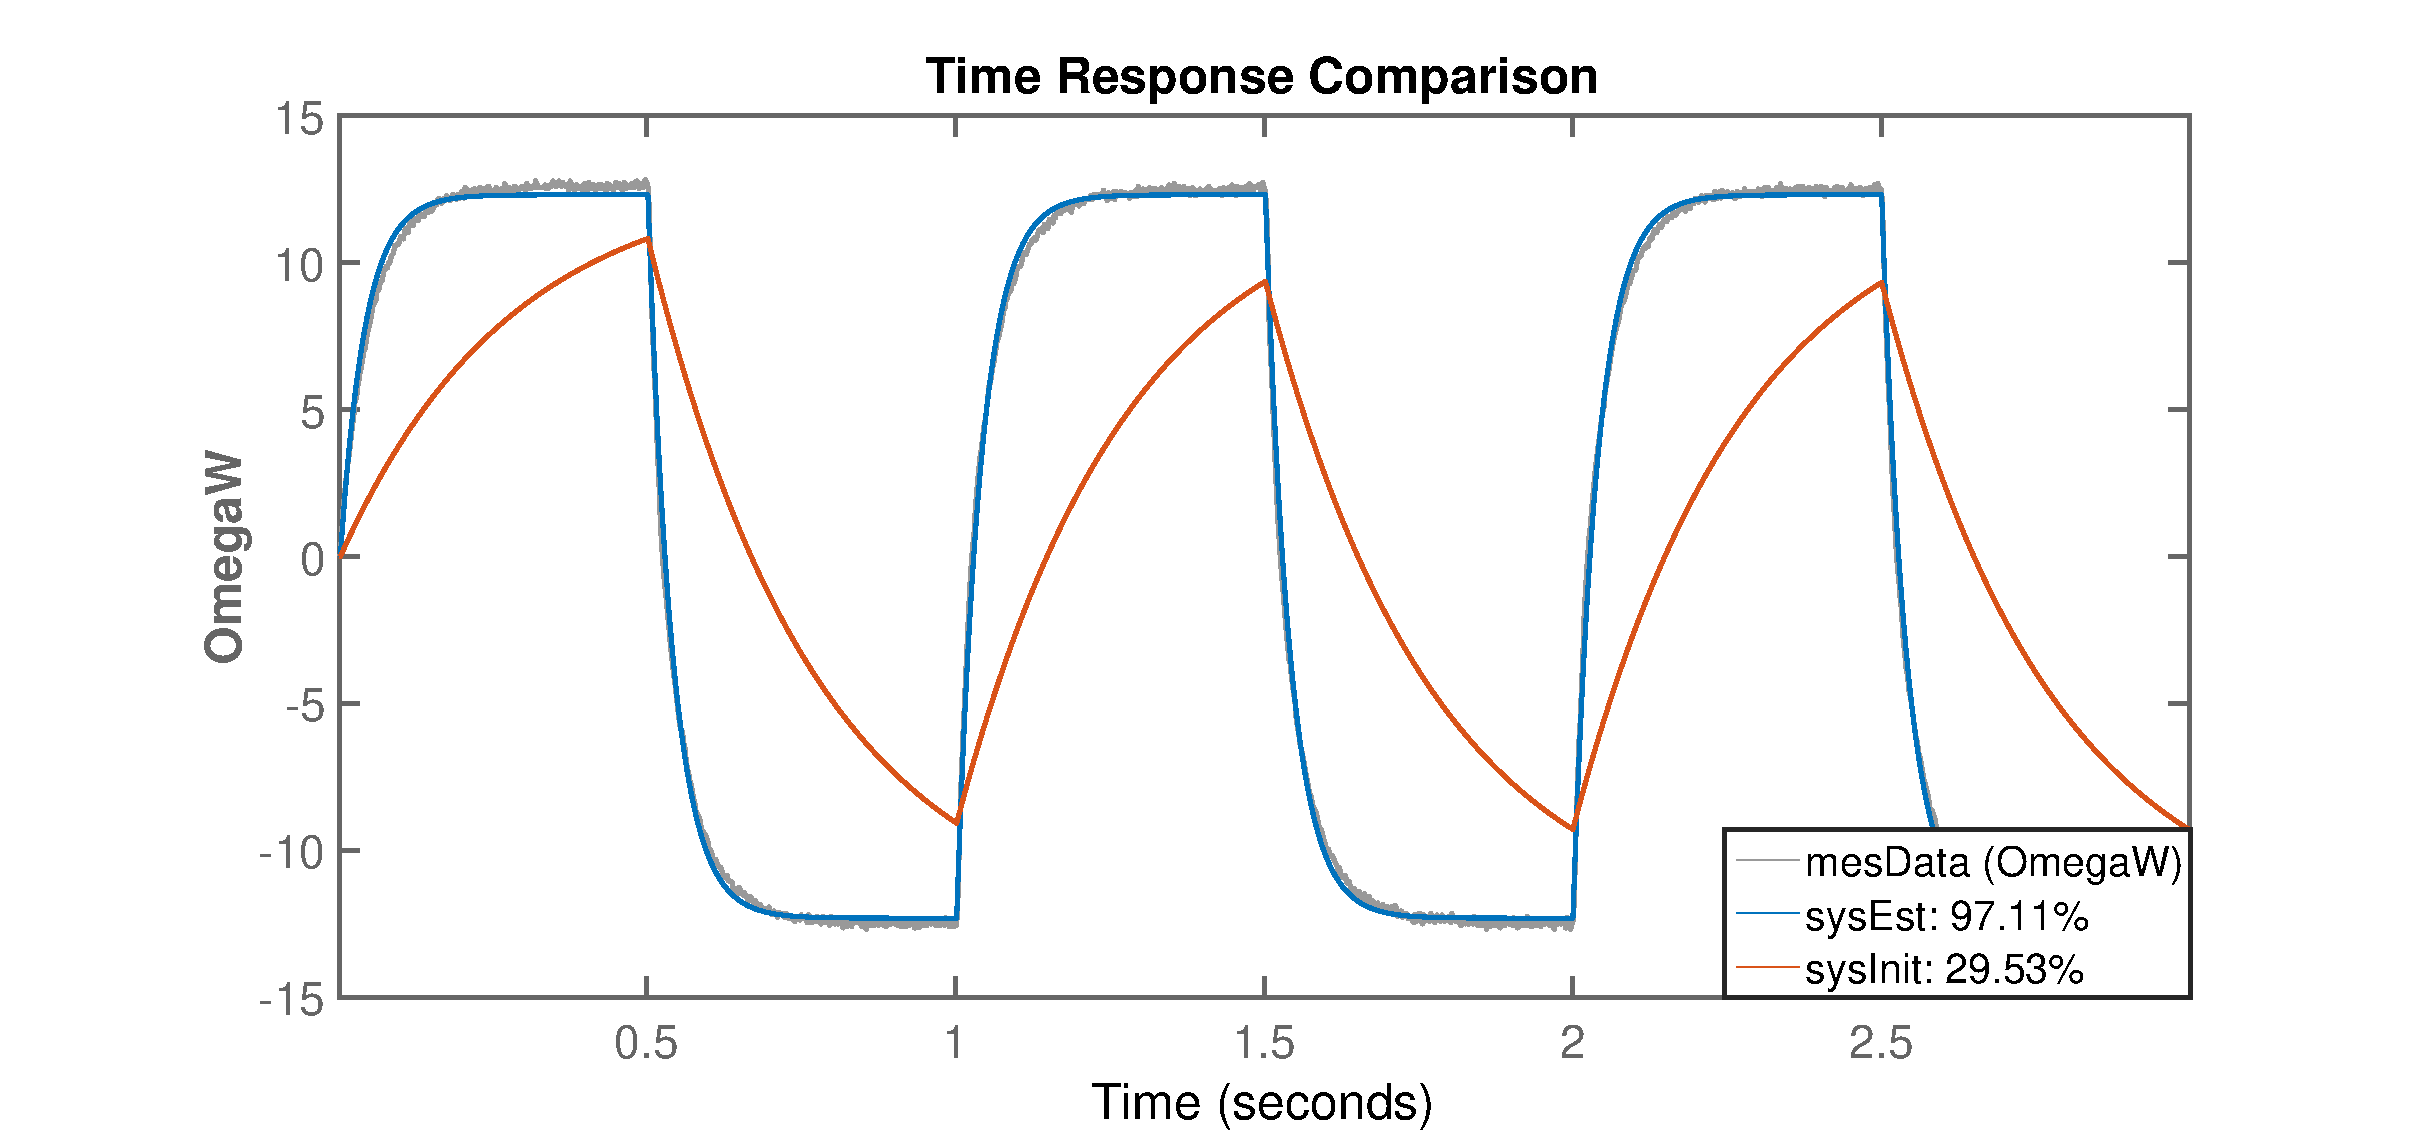
\includegraphics[width = \textwidth]{ParameterEstimation.eps}
    \caption{Bode plot of the transfer function for the segway.}
    \label{fig:paramEst1}
\end{figure} 

With the new gain, the response can be seen in \autoref{fig:paramEst1}, where the model prediction, shown in orange, is shown together with the measured data in grey. The blue axis is Matlab's estimate, based on the model type and measured data.

The model provided by matlab is tested on a different data set, where the motor voltage is changed from 1,96 V to -3,92 V. This can be seen in \autoref{fig:segwayBode_Merge}, where a correlation between the model and the data of $83 \% $ is obtained.

\begin{figure}[H]
    \centering
    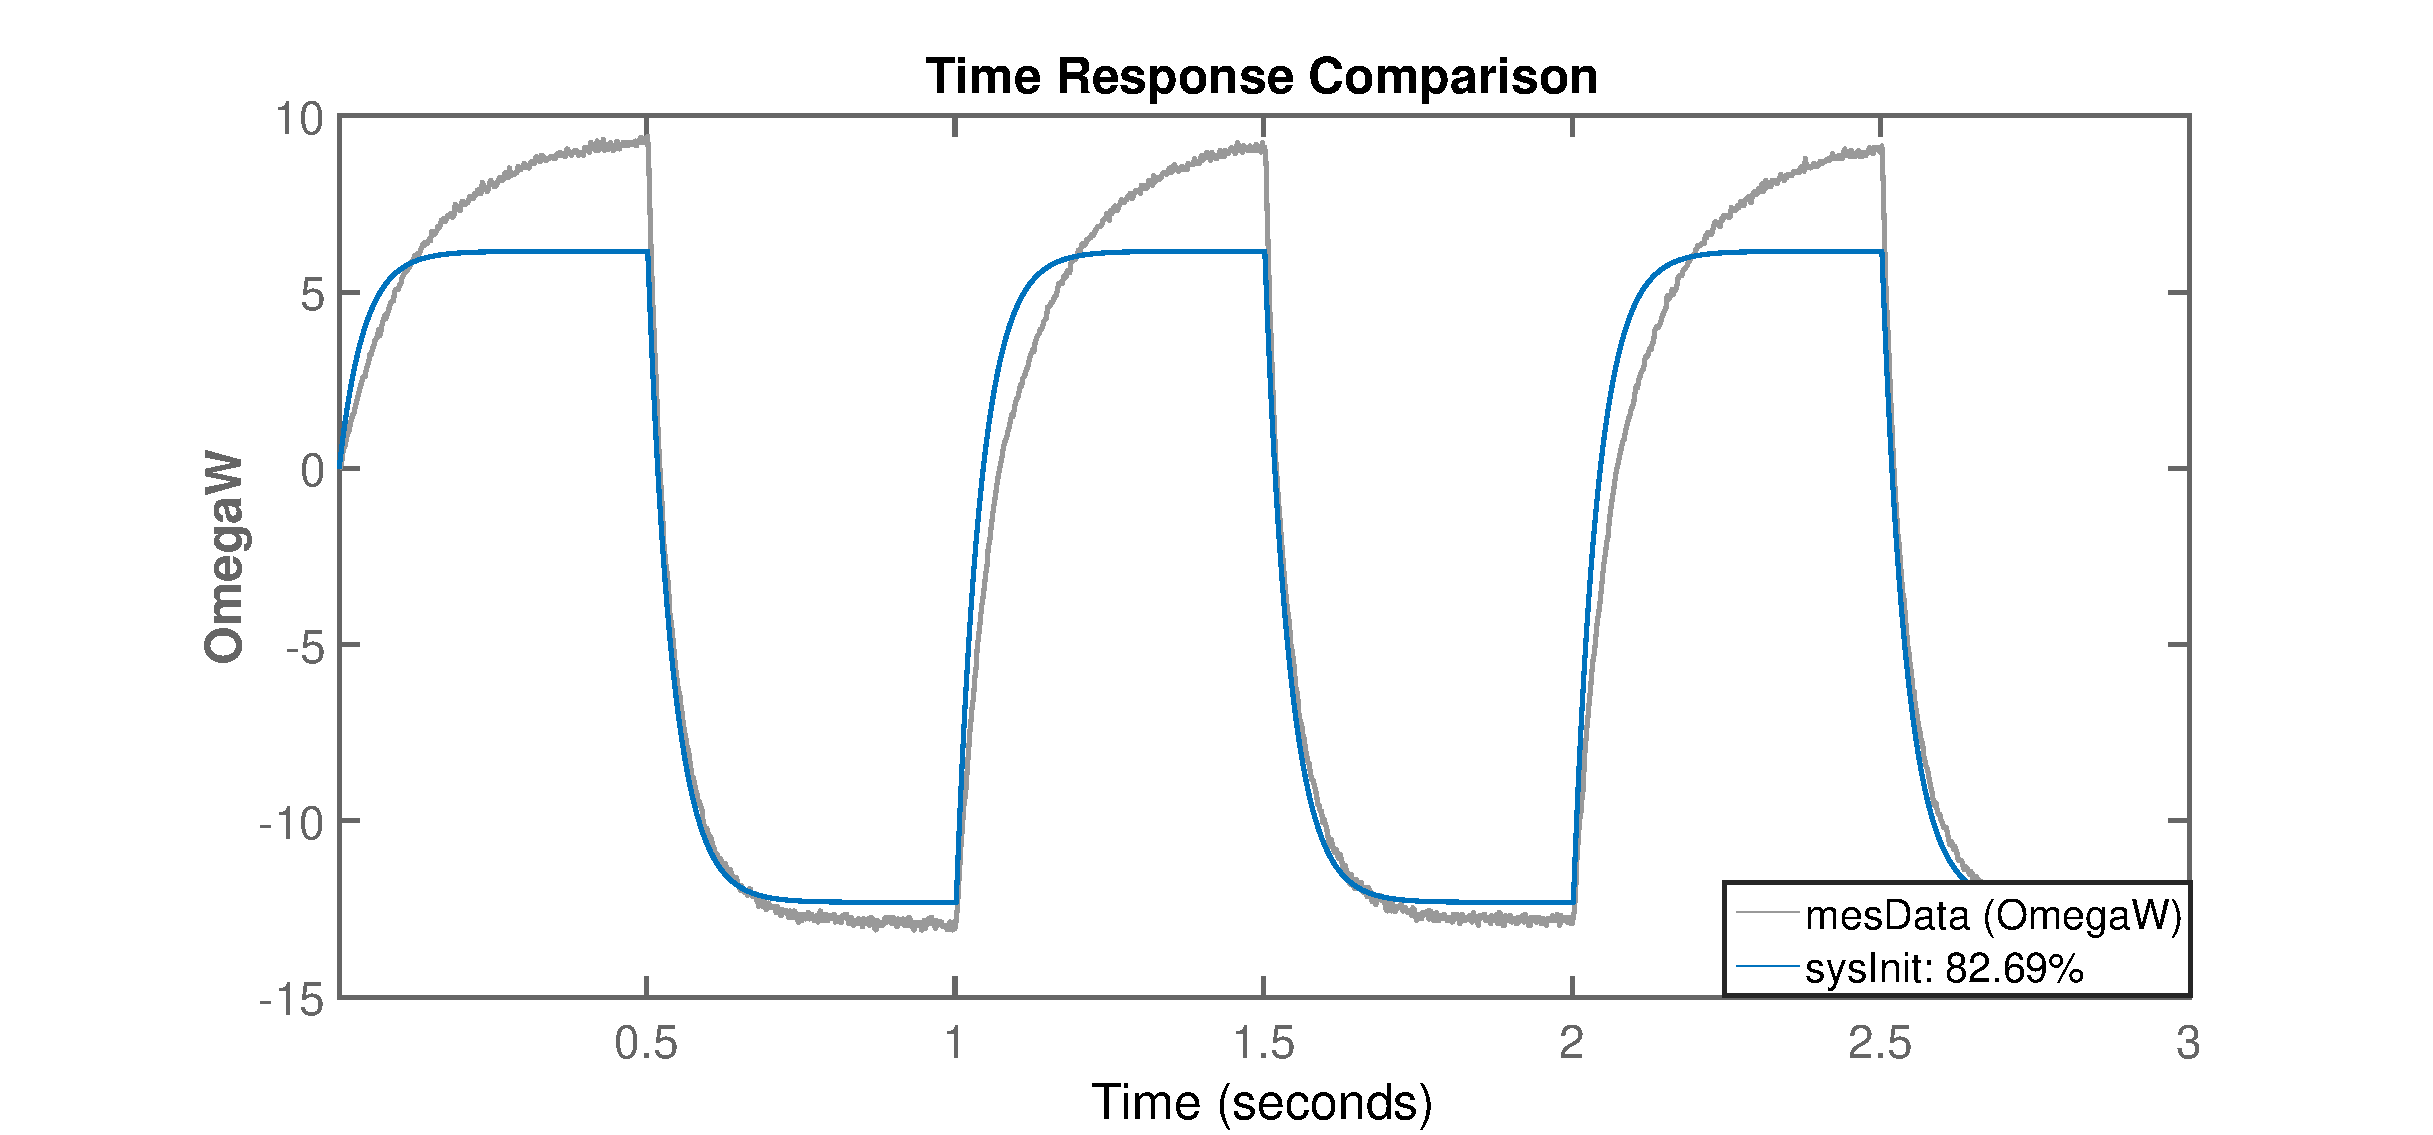
\includegraphics[width = \textwidth]{EstimationTest.eps}
    \caption{Bode plot of the transfer function for the segway.}
    \label{fig:paramEst2}
\end{figure} 

This is assumed to be satisfying, and thus the model for the motors and wheels has been found. Note that in the test, it is the transfer function $\frac{\omega_w{s}}{V_a(s)}$ that has been found, and thus the relationship between $\omega_w$ and $F_F$ as stated in \autoref{OmegaToForce} has to be taken into account. Doing this, results in the following transfer function:

\begin{equation}
\frac{F_F(s)}{V_a(s)} = \frac{0.049s}{0.040s + 1}
\label{eq:motorWheelFinal}
\end{equation}


\section{Model of Cart and Inverted Pendulum \label{sec:pen_model}}
In this section, a model of the inverted pendulum is derived. This model describes the movement of the cart and the inverted pendulum, based on governing equations put up regarding the behaviour of the system. To do this, it is necessary to investigate how the inverted pendulum moves, and how the interaction between the inverted pendulum and the cart can be described. Before this is done in detail, it is however first necessary to obtain an overview of the inverted pendulum.
\subsection{Overview of the Inverted Pendulum}
The model of the inverted pendulum describes how the two masses, i.e. the cart and the inverted pendulum, behaves when a force is exerted upon it by the surroundings. Note that the rod connecting the inverted pendulum mass to the cart is assumed massless, and is therefore not a part of the model. A schematic drawing of the inverted pendulum is shown in \autoref{fig:mecmodinvpen}.
\begin{figure}[H]
\centering
%\includegraphics[scale=1]{needstobechaged1.png}
\scalebox{0.6}{\input{figures/invpenmec.ralf}}
\caption{Mechanical model of the inverted pendulum.}
\label{fig:mecmodinvpen}
\end{figure}
In \autoref{fig:mecmodinvpen} the mass at the end of the rod is $m_p$, the variable $\theta_p(t)$ describes the angle of the inverted pendulum from a vertical line at the center of the cart. Note that the angle is positive in the counter-clockwise direction. This angle can be described in relation to both the x- and y-direction. The force applied to move the segway is labelled $F_F(t)$.\\\\
For simplicity, the coordinate system is defined such that $y_c(t)$ is 0, thus:
\begin{align}
x_p(t)&= x_c(t)- l \cdot \sin(\theta_p(t))\\
y_p(t)&= l\cdot \cos(\theta_p(t)) 
\end{align}
\begin{where}
\va{$x_p(t)$}{is the x-position of the inv. pendulum}{m}\\
\va{$x_c(t)$}{is the x-position of the cart}{m}\\
\va{$l$}{is the length between the center of rotation of the cart and the center of mass of the inv. pendulum}{m}\\
\va{$\theta_p(t)$}{is the angle of the inv. pendulum}{rad}\\
\va{$y_p(t)$}{is the y-position of the inv. pendulum}{m}\\
\end{where}

From this, the accelerations can be found by taking the double time differential of both sides of the above equations:
\begin{align}
\ddot x_p(t) &= \ddot x_c(t) + l \cdot \sin(\theta_p(t))\cdot \dot\theta_p^2 (t) - l \cdot \cos(\theta_p(t))\cdot \ddot\theta_p(t) \label{eq_acc_x}\\
\ddot y_p(t) &= -l\cdot \cos(\theta_p(t)) \cdot \dot\theta_p^2 (t) - l \cdot \sin(\theta_p(t))\cdot \ddot\theta_p (t)\label{eq_acc_y}
\end{align}
\begin{where}
\va{$\ddot x_p(t)$}{is inv. pendulum's acceleration in the x-direction }{rad/$\text{s}^2$}\\
\va{$\ddot \theta_p(t)$}{is inv. pendulum's angular acceleration}{rad/$\text{s}^2$}\\
\va{$\dot \theta_p(t)$}{is inv. pendulum's angular velocity}{rad/s}\\
\va{$\ddot y_p(t)$}{is inv. pendulum's acceleration in the y-direction }{rad/$\text{s}^2$}\\
\end{where}
%To make a transfer function for the inverted pendulum that can be merged with the transfer function for the motors and wheels, an equation in time domain describing the change in $\theta_p(t)$ caused by any $F_F(t)$ must first be derived. This is done in the following section.

To derive a model expression for the inverted pendulum, which shall be combined with a model expression for the motors and wheels, an equation %in time domain 
 describing the change in $\theta_p(t)$ caused by any $F_F(t)$ must first be derived. This is done in the following section.
\subsection{Equations of Motion}
In this section, translatoric free body diagrams for the cart and the inverted pendulum are presented and used to derive equations of motion. From these, a model of the cart and the inverted pendulum can be obtained.
 %\todo{is it still the only purpose, i think it has changed.A}The goal of this section is to arrive at one expression with only two variables, namely the input, $F_F(t)$ and the output, $\theta_p(t)$ of the model for the inverted pendulum. %Subsequently this expression is verified through simulation, and comparison with expected result.
\newpar
From \autoref{fig:mecmodinvpen}, free body diagrams can be determined. In this case, the cart's and the inverted pendulum's free body diagrams are representing the forces acting upon them while the segway is at an angle, $\theta_p(t)$.\\
The free body diagram of the mass at the end of the rod, is shown in \autoref{fig:fbdm1}.
\begin{figure}[H]
%\hspace{-0.5 cm}
\centering
\begin{subfigure}[b]{0.42\textwidth}
		\hspace{1.5cm}
        \scalebox{0.6}{\input{figures/invpen_M2_FBD.ralf}}
        %\vspace{3mm}
		\caption{FBD of the cart.}
		\label{fig:fbdm2}
\end{subfigure}
\hspace{1 cm}
\begin{subfigure}[b]{0.42\textwidth}
		\centering
        \scalebox{0.6}{\input{figures/invpen_M1_FBD.ralf}}
        %\vspace{10 mm}		
		\caption{FBD of the pendulum mass.}
		\label{fig:fbdm1}
    \end{subfigure}  
\caption{Free body diagrams of the mass of the inverted pendulum and the mass of the cart.}
\label{fig:FBDMotorWheel}
\end{figure}
\clearpage
The forces acting on the the mass $m_p$ is the gravitational force $F_g$, and the tension in the rod between the cart and the inverted pendulum, $F_t(\theta_p(t))$. This force is split up into two composants - a composant in the x-direction, $F_{tx}(\theta_p(t))$ and one in the y-direction, $F_{ty}(\theta_p(t))$. % The magnitude of this force depends on the angle, $\theta_p(t)$.\\
\autoref{fig:fbdm2} shows the free body diagram of the segway's cart. The force $F_g$ is the gravitational force and $F_N$ is the force pushing upwards from the ground. Note that the magnitude of the tension force $F_t(\theta_p(t))$ is equal to the force acting upon the inverted pendulum, but in opposite direction. %Furthermore, the force $F_F(t)$ from \autoref{fig:mecmodinvpen} has been split in two forces, namely $F_{F1}$ and $F_{F2}$, because there are two motors applying this force. The forces $F_{F1}$ and $F_{F2}$ have the same direction and magnitude, as it is assumed that the motors apply the same force to the system. \newpar
From the free body diagrams, it is now possible to express the dynamics of the inverted pendulum with the following three equations of motion. \\\\
For the inverted pendulum:
\begin{align}
m_p \cdot \ddot x_p(t) &= - F_{tx}(\theta_p(t)) \label{eom1}\\
m_p \cdot \ddot y_p(t) &= F_{ty}(\theta_p(t)) - F_g \label{eom2}
\end{align}
\begin{where}
\va{$m_p$}{is the mass of the inv. pendulum}{kg}\\
\va{$\ddot x_p(t)$}{is inv. pendulum's acceleration in the x-direction}{$\text{m}/\text{s}^2$}\\
\va{$F_{ty}(\theta_p(t))$}{is the rod's tension force in the y-direction}{N}\\
\va{$F_{tx}(\theta_p(t))$}{is the rod's tension force in the x-direction}{N}\\
\va{$\theta_p(t)$}{is inv. pendulum's angle from cart's center}{rad}\\
\va{$\ddot y_p(t)$}{is inv. pendulum's acceleration in the y-direction}{$\text{m}/\text{s}^2$}\\
\va{$F_g$}{is the gravitational force}{N}\\
\end{where} 

Note that \autoref{eom1} is for the horizontal direction and \autoref{eom2} is for the vertical direction. For the cart, it is only relevant to sum the forces in the horizontal direction, as it is assumed that the surface the cart moves on is immovable. 
\begin{align}
m_c \cdot \ddot x_c(t) = F_{tx}(\theta_p(t))+ F_{F}(t)\label{eom3}
\end{align}
\begin{where}
\va{$m_c$}{is the mass of the cart}{kg}\\
\va{$\ddot x_c(t)$}{is the cart's acceleration in the x-direction}{$\text{m}/\text{s}^2$}\\
\va{$F_{F}(t)$}{is the applied force from the motors}{N}\\
\end{where}

From equation \autoref{eom3} it can be deducted that the load force $F_L$ is equivalent to $F_{tx}$ since this is the contribution from the inverted pendulum. By combining \autoref{eq_acc_y}, \ref{eom1} and \ref{eom3} the governing equation for cart's movement can be obtained.
\begin{equation}
m_c \cdot \ddot x_c(t) = F_{F}(t) - m_p\left(\ddot x_c(t) + l \cdot \sin(\theta_p(t))\cdot \dot\theta_p^2(t) - l \cdot \cos(\theta_p(t))\cdot \ddot\theta_p(t)\right)\label{eq:model_pen33}
\end{equation}

From this, it can be seen that the load force can be described as:
\begin{equation}
F_L = m_p\left(\ddot x_c(t) + l \cdot \sin(\theta_p(t))\cdot \dot\theta_p^2(t) - l \cdot \cos(\theta_p(t))\cdot \ddot\theta_p(t)\right)
\label{loadForce}
\end{equation}
%Note that from this, the load torque to the motors can be found. 
%\autoref{eq:model_pen33} states that the resultant force acting on the cart is equal to the applied force, minus the contribution from the pendulum, which is the last term in \autoref{eq:model_pen33}. Thus, if the resultant force is to be the same as the applied, the motor is to overcome the contribution from the pendulum. In this respect, the last term in \autoref{eq:model_pen33} can be seen as the load torque to the motors, when multiplied with the wheel radius, i.e.:
%\begin{equation}
%\tau_L(t) = r_w \cdot m_p\left(\ddot x_c(t) + l \cdot \sin(\theta_p(t))\cdot \dot\theta_p^2(t) - l \cdot \cos(\theta_p(t))\cdot \ddot\theta_p(t)\right) 
%\label{tauLDef}
%\end{equation}

%The equations of motion for both the pendulum and the cart are all translatoric. To eliminate the variables $\ddot x_1(t)$ and $\ddot y_1(t)$ kinematics is applied. From the principles  of kinematics the equations of motion can be expressed in only rotational terms. The acceleration of the pendulum is a sum of the acceleration of the pendulum in relation to the cart and the acceleration of the cart.

Now, the translatoric movement of the inverted pendulum has been described, and the rotation thus needs to be described. The rotation of the inverted pendulum is described from the resultant torque acting on the inverted pendulum, denoted as $J_p \ddot{\theta_p}(t)$. The rotation of the inverted pendulum occurs around the center of mass of the inverted pendulum. From \autoref{torqueDeriviation}, it can be seen that there are three forces determining the rotation of the inverted pendulum, namely the gravitational force, $F_g$, and the x- and y-composants of the tension force, namely $F_{tx}$ and $F_{ty}$.

\begin{figure}[H]
\centering
\scalebox{0.6}{\input{figures/modellingSeg.ralf}}
%\input{figures/modellingSeg.ralf}
\caption{The forces contributing to the resultant torque of the inverted pendulum.}
\label{torqueDeriviation}
\end{figure}

The mentioned forces exert a torque on the inverted pendulum based on their distance from the center of rotation. In the case of the segway, the arm is the length of the rod, where the forces acting upon it are $F_{tx}$ and $F_{ty}$. It can be seen that $F_g$ attacks at the point mass, resulting in the arm length being zero and is therefore not acting upon the inverted pendulum. 
It should be noted that it is only the composant of the forces which are perpendicular to the rod that contributes to the torque, which needs to be included in the torque expressions. 
Thus, summing over the torques, the resultant pendulum torque can be described as:

\begin{equation}
J_p \ddot{\theta_p}(t) =  l \cdot \sin(\theta_p) F_{ty}-l \cdot \cos(\theta_p) F_{tx} \label{eq:gov2}
\end{equation}
\begin{where}
\va{$J_p$}{is the inertia of the inverted pendulum}{kg $m^2$}\\
\end{where}

A governing equation for the inverted pendulum can be obtained by inserting \autoref{eq_acc_x} in \autoref{eom1} and \autoref{eq_acc_y} in \autoref{eom2} and inserting these expressions in \autoref{eq:gov2}:
\begin{align}
\begin{split}
J_p \ddot{\theta_p}(t) &= m_p \cdot l \cdot \sin(\theta_p(t))\left(g -l \cdot \cos(\theta_p(t))\cdot \dot \theta_p^2(t) - l \cdot \sin(\theta_p(t)) \cdot \ddot \theta_p(t)\right)\\&+m_p \cdot l \cdot \cos(\theta_p(t))\left(\ddot x_c(t) - l \cdot \sin(\theta_p(t))\cdot \dot \theta_p^2(t) - l \cdot \cos(\theta_p(t)) \cdot \ddot \theta_p(t)\right)
\end{split}
\end{align}

Expanding this and using simple geometric relations, the expression can be simplified to:
\begin{equation}
(J_p+m_p\cdot l^2)\cdot \ddot \theta_p(t) = m_p \cdot l \cdot \left(\sin(\theta_p(t)) \cdot g+ \cos(\theta_p(t)) \cdot \ddot x_c(t)\right) \label{eq:inertia1}
\end{equation}

%The acceleration of the pendulum in relation to the cart can only be in a circle around the cart. The pendulums acceleration around the circle, is the sum of two accelerations. Namely the tangent acceleration in the direction described by $\vv{\epsilon_\theta}$ and the centripetal acceleration in the direction described by $\vv{\epsilon_r}$ and shown in \autoref{fig:invPenKin}
%Thus the acceleration of the pendulum can be expressed as \autoref{eom4}.
%
%\begin{figure}[H]
%\centering
%\scalebox{0.6}{\input{figures/invpenmec_kin.ralf}}
%\caption{Mechanical model of the inverted pendulum with the direction of the centripetal acceleration and the tangent acceleration.}
%\label{fig:invPenKin}
%\end{figure}
%
%\begin{align}
%\vv{a_p} = l\cdot \ddot \theta(t)\cdot \vv{\epsilon_\theta} + l \cdot \dot \theta(t) ^2 \cdot \vv{\epsilon_r} + \ddot x_c = \vv{a_{p/c}}+\vv{a_c} \label{eom4}
%\end{align}
%\begin{where}
%\va{$\vv{a_p} $}{is the vector describing the acceleration of the pendulum}{$\frac{\text{m}}{\text{s}^2}$}\\
%
%\va{$\vv{\epsilon_\theta}$}{is the vector describing the direction of the tangent acceleration}{1}\\
%\va{$\dot\theta(t)$}{is the angular velocity}{$\frac{\text{rad}}{\text{s}}$}\\
%\va{$\vv{\epsilon_r}$}{is the vector describing the direction of the centripetal acceleration}{1}\\
%\va{$\vv{a_{p/c}}$}{is the vector describing the acceleration of the pendulum relative to the cart}{$\frac{\text{m}}{\text{s}^2}$}\\
%\va{$\vv{a_c}$}{is the vector describing the acceleration of the cart}{$\frac{\text{m}}{\text{s}^2}$}
%\end{where}
%
%Expanding \autoref{eom4}'s vectors, so the accelerations are expressed in terms of the x- and y-directions, will give the following two equations.
%\begin{align}
%\ddot x_p(t)&=\vv{a_{px}}= -l \cdot \ddot\theta_p(t)\cdot \cos(\theta_p(t)) + l \cdot \dot \theta_p(t)^2 \cdot \sin(\theta_p(t))+\ddot x_c(t)  \label{eom5} \\
%\ddot y_p(t)&=\vv{a_{py}}=-l\cdot \ddot\theta_p(t)\cdot\sin(\theta_p(t)) - l \cdot \dot \theta_p(t)^2 \cos(\theta_p(t))-g\label{eom6}
%\end{align}
%
%\begin{where}
%\va{$\vv{a_{px}}$}{is the vector describing the pendulums acceleration in the x-direction}{$\frac{\text{m}}{\text{s}^2}$}\\
%\va{$\vv{a_{py}}$}{is the vector describing the pendulums acceleration in the y-direction}{$\frac{\text{m}}{\text{s}^2}$}
%\end{where}
%
%
%$\ddot x_p(t)$ and $\ddot y_p(t)$ is eliminated, by inserting \autoref{eom5} into \autoref{eom1} and \autoref{eom4} into \autoref{eom2}, yielding \autoref{eom7} and \autoref{eom8} respectively.
%
%\begin{align}
%-m_p\cdot l\cdot \ddot \theta_p(t) \cdot \cos(\theta_p(t))+m_p \cdot l\cdot \dot \theta_p^2(t) \cdot \sin(\theta_p(t))+m_p\cdot \ddot x_c(t)= - F_t(\theta_p(t)) \cdot \sin(\theta_p(t)) \label{eom7}
%\end{align}
%\begin{align}
%-m_p \cdot l \cdot \ddot \theta_p(t)\cdot\sin(\theta_p(t)) - m_p \cdot l\cdot \dot \theta_p^2(t) \cdot \cos(\theta_p(t))= F_t(\theta_p(t)) \cdot \cos(\theta_p(t)) - m_p \cdot g \label{eom8}
%\end{align}
%
%\begin{where}
%\va{$g$}{is the gravitational acceleration}{$\frac{\text{m}}{\text{s}^2}$}\\
%\end{where}
%
%\begin{figure}[H]
%\centering
%\includegraphics[width =0.3 \textwidth]{figures/inertia11.jpg}
%\caption{Tension force composants.}
%\label{fig:NewFig}
%\end{figure}
%
%From \autoref{fig:NewFig}, it can be seen that the tension force $F_t(\theta_p(t))$ can be slit into two composants, i.e. two forces perpendicular to each other. These can be described as:
%\begin{align}
%F_{t, x}(\theta_p(t)) &= - F_t(\theta_p(t)) \cdot \sin(\theta_p(t))\\
%F_{t, y}(\theta_p(t)) &= F_t(\theta_p(t)) \cdot \cos(\theta_p(t))
%\end{align}
%
%These forces can be used to obtain an expression for the resultant torque acting on the pendulum. From \todo{source: matlab} it can be seen that the following relation applies:
%
%\begin{equation}
%J_p \ddot \theta_p(t) = - F_{t, x}(\theta_p(t)) \cdot l \cdot \cos(\theta_p) - F_{t, y}(\theta_p(t)) \cdot l \cdot \sin(\theta_p)
%\label{inertiaLink}
%\end{equation}
%
%By multiplying \autoref{eom7} with $\cos(\theta_p(t))$ and \autoref{eom8} with $\sin(\theta_p(t))$ then adding the two equations, the expression for the inertia as described in \autoref{inertiaLink} can be utilized, yielding \autoref{eom9}.
%
%Multiply with $l \cdot \cos(\theta)$ on both sides in \autoref{eom7}:
%\begin{align}
%-m_p\cdot l^2 \cdot \ddot \theta_p(t) \cdot \cos^2 (\theta_p(t))+m_p\cdot l^2 \cdot \dot \theta_p^2(t) \cdot \sin(\theta_p(t))\cdot \cos(\theta_p(t))+m_p\cdot l \cdot \ddot x_c \cdot \cos(\theta_p(t)) = F_{t, x}(\theta_p(t)) \cdot l \cdot \sin(\theta_p(t))\label{eom9}
%\end{align}
%
%Multiplying with $l \cdot \sin(\theta)$ on both sides in \autoref{eom8}:
%\begin{align}
%-m_p\cdot l^2 \cdot \ddot \theta_p(t)\cdot \sin^2 (\theta_p(t)) - m_p\cdot l^2 \cdot \dot \theta^2(t) \cdot \cos(\theta_p(t))\cdot \sin(\theta_p(t))=-m_p \cdot l \cdot g\cdot \sin(\theta_p(t)) - F_{t, y}(\theta_p(t)) \cdot l\cdot \sin(\theta_p(t)) \label{eom10}
%\end{align}
%
%Adding \autoref{eom9} and \autoref{eom10} and using the expression for the :
%
%
%
%To eliminate $\ddot x_c(t)$, an equation containing only the variables $\ddot x_c(t)$, $F_F$ and $\theta_p(t)$ and its derivatives must be constructed. This is done by substituting the left side of \autoref{eom7} into \autoref{eom3} in place of $F_t(\theta_p(t)) \cdot sin(\theta_p(t))$. This yields \autoref{eom10}.
%\begin{align}
%(m_p+m_c)\cdot \ddot x_c(t)=m_p\cdot l\cdot \ddot \theta_p(t) \cdot \cos(\theta_p(t))-m_p\cdot l\cdot \dot \theta_p(t)^2 \cdot \sin(\theta_p(t))+F_F(t)\label{eom10}
%\end{align}
%
%With 2 equations containing $\ddot x_c(t)$, this variable is now eliminated by isolating $\ddot x_c(t)$ in \autoref{eom9} and inserting this expression for $\ddot x_c(t)$ in \autoref{eom10}. This yields \autoref{eq:thetaForce}.
%\begin{align}
%\ddot \theta_p(t)(l\cdot (m_p + m_c)-m_p \cdot l \cdot \cos^2(\theta_p(t)))&+\dot\theta_p(t)^2 \cdot (m_p\cdot l\cdot \sin(\theta_p(t))\cdot \cos(\theta_p(t)))\nonumber\\ 
%&=  \\
%\cos(\theta_p(t))\cdot F_F(t)+g\cdot &\sin(\theta_p(t))\cdot (m_p+m_c)\nonumber\label{eq:thetaForce}
%\end{align}
%
%\autoref{eq:thetaForce} contains only two variables, namely $\theta_p(t)$ and $F_F(t)$, thus this single expression describes the motion of the inverted pendulum. This model is clearly not linear, thus it has to be linearised before a transfer function can be determined. This is done in the next subsection.
%
%%In the following section, a block diagram is build from this expression, through which the expression is verified by simulation and subsequent comparison with expected result.
%%changed due to mistak where L was not included.
%%\begin{align}
%%\ddot \theta (-m_1\cdot L \cdot \cos^2(\theta)+(m_1+m_2)\cdot L)+\dot \theta^2(m_1\cdot \sin(\theta)\cdot \cos(\theta))=F_F+(m_1+m_2)\cdot g\cdot \sin(\theta)
%%\end{align}
%The model of the inverted pendulum without the inertia can be expressed as: 
%\begin{equation}
%(m_p+m_c)\cdot \ddot x_c(t)= m_p\cdot l \cdot \ddot \theta_p(t) \cdot \cos(\theta_p(t))-m_p \cdot l \cdot \dot \theta_p(t)^2 \sin(\theta_p(t))+2\cdot F_F(\theta_p(t))\label{eq:penmodelnoinertia}
%\end{equation}
%
%Note, that $F_F(\theta_p(t))$ is multiplied by two, as there are two wheels applying force. \\
%This expression can be combined with \autoref{eq:inertia1}. 
%This is done by isolating $\ddot x_c(t)$ in \autoref{eq:penmodelnoinertia}. Inserting this into \autoref{eq:inertia1} yieds: 
%\begin{align}
%&(J_p+m_p\cdot l^2)\cdot (m_p + m_c)\cdot \ddot \theta_p(t)=(m_p^2 +m_p\cdot m_c)\cdot l \cdot g \cdot \sin(\theta_p(t))\nonumber \\&+m_p^2\cdot l^2\cdot \cos^2(\theta_p(t)) \cdot \ddot \theta_p(t)-m_p\cdot l \cdot \dot \theta_p(t)^2\cdot \sin(\theta_p(t))+2\cdot F_F(\theta_p(t))\label{eq:final_pen22}
%\end{align}
\autoref{eq:model_pen33} and \autoref{eq:inertia1} are the final model expressions for the inverted pendulum. The next step before transfer functions are derived, is to linearize these expressions. This is done in the following section.
\vspace{1 cm}
%This can now be combined with the model expression of the motors and wheels model. This is done in the following section. 
% This will be linearized in the following section and combined with the already linear motormodel. This will lead to a transferfunction for the system, which is to be simulated. From this a controller can be designed and later implemented. 
%\input{design/modelling/Inv_pen_model_non_lin.tex}
\section{Derivation of Segway Transfer Functions}
In this section, the model expressions derived in previous sections are verified, linearized and combined into transfer functions. From these transfer functions, the controllers will be designed to allow the segway to balance in an upright position. In this section, the models are viewed and linked as illustrated in \autoref{fig:modelOverallLin}.
\begin{figure}[H]
\centering
\begin{tikzpicture}[auto, node distance=3.5cm,>=latex']
    % We start by placing the blocks
    \node [input, name=input] {};

    % Once the nodes are placed, connecting them is easy. 
	\draw[thick,dashed, fill=black!10, align=center] ($(input.north west)+(15.5,-1)$) rectangle ($(input.north west)+(0.6,2.75)$);
	\draw[thick,dashed, fill=black!30, align=center] ($(input.north west)+(10.75,-0.8)$) rectangle ($(input.north west)+(1.5,1.75)$);
	 \node [align=center] at ($(input.north west)+(8,2.25)$) {\textbf{Plant, }$\mathbf{ \, \, \, G}$};
	 \node [align=center] at ($(input.north west)+(6,1.25)$) {{Motors and Wheels Model}};
	
	\node [blockbig, right of=input, align = center] (motor) {Motor \\ and Wheel};
	\node [blockbig, right of=motor, align = center, node distance=4.5cm] (Cart) {Cart \\ Movement};
    \node [blockbig, right of=Cart, align = center, node distance=4.5cm] (pendulum) {Inverted \\ Pendulum};

   \node [output, right of=pendulum, node distance=3.5cm] (output) {};

	
    \draw [->] (input) -- node {$V_a$} (motor);
    \draw [->] (4.75,0.2) -- node {$\tau_a$} (6.75,0.2);
    \draw [->] (9.25,0.2) -- node {$\theta_w$} (11.25,0.2);
    \draw [->] (11.25,-0.2) -- node {$F_L$} (9.25,-0.2);
   % \draw [->] (9.75,-0.2) -| node {} (3.75,-0.2);
    \draw [->] (pendulum) -- node {$\theta_p$} (output);
\end{tikzpicture}
\caption{Block diagram of the plant, also known as system model.}
\label{fig:modelOverallLin}
\end{figure}
Note that the models are linked differently than previously shown in \autoref{fig:modelOverall}, since the cart movement is made part of the motor and wheel model, instead of being part of the inverted pendulum model. This is because it is not possible to measure the torque $\tau_a$, while the wheel angle, $\theta_w$, can be measured by the encoders. Thus, it will be possible to derive a transfer function for the motors and wheels model. The same applies for the inverted pendulum model, where it will be possible to derive and verify a transfer function based on an input being the wheel angle, $\theta_w$, instead of the torque $\tau_a$.
\subsection{Verification of Models}
The three model expressions that have been derived in the previous sections are \autoref{eq:MotorFinal}, \ref{eq:model_pen33} and \ref{eq:inertia1}. For repetition, these are shown below.
\begin{align}
\tau_a(t) = \frac{1}{N_{ms} N_{sw}}\Big(\frac{k_t}{R_a} \big( V_a(t)& - k_e \dot\theta_m(t) \big) - \ddot\theta_m(t)J_{T} - \dot\theta_m(t)B_{T}\Big)
\label{eq:model3}\\
m_c \cdot \ddot x_c(t) = F_F(V_a(t)) - m_p\Big(\ddot x_c(t)& + l \cdot \sin(\theta_p(t))\cdot \dot\theta_p^2(t) - l \cdot \cos(\theta_p(t))\cdot \ddot\theta_p(t)\Big)\label{eq:model2}\\
(J_p+m_p\cdot l^2)\cdot \ddot \theta_p(t) = m_p \cdot l \cdot &\left( \sin(\theta_p(t)) \cdot g+\cdot \cos(\theta_p(t)) \cdot \ddot x_c(t) \right) \label{eq:model1}
\end{align}

If no slip is assumed in the gearing and between the wheels and the ground, then $\dot \theta_m(t)$ and $\ddot \theta_m(t)$ can be replaced with $N_{ms}N_{sw} \cdot \dot \theta_w(t)$ and $N_{ms}N_{sw} \cdot \ddot \theta_w(t)$ respectively, and $\ddot x_c(t)$ can be replaced with $r_w \cdot \ddot \theta_w(t)$. This yields the three governing equations for the system model:
\begin{align}
\tau_a(t) =\frac{\left( \frac{K_t}{R_a} \left( V_a(t) - \frac{K_e }{N_{ms} N_{sw}} \cdot \dot\theta_w(t) \right) - \frac{J_{T}}{N_{ms} N_{sw}} \cdot \ddot\theta_w(t) - \frac{B_{T}}{N_{ms} N_{sw}} \cdot \dot\theta_w(t) \right)}{N_{ms} N_{sw}}
\label{eq:model3W}\\
m_c \cdot r_w \cdot \ddot \theta_w(t) = F_F(V_a(t)) - m_p\left(\ddot \theta_w(t) \cdot r_w + l \cdot \sin(\theta_p(t))\cdot \dot\theta_p^2(t) - l \cdot \cos(\theta_p(t))\cdot \ddot\theta_p(t)\right)\label{eq:model2W}\\
(J_p+m_p\cdot l^2)\cdot \ddot \theta_p(t) = m_p \cdot l \cdot \left( \sin(\theta_p(t)) \cdot g+\cdot \cos(\theta_p(t)) \cdot r_w \cdot \ddot \theta_w(t) \right) \label{eq:model1W}
\end{align}

To form the governing equation for the motors and wheels model, \autoref{eq:model3W} and \autoref{eq:model2W} are to be combined, see \autoref{fig:modelOverallLin}. 
To meet the interfaces specified, see \autoref{fig:modelOverallLin}, the relation between the motor and wheel model's output $\tau_a(t)$ and the force $F_F(t)$ which the cart movement model has as input, see \autoref{eq:model3W}, must be determined. 

There are two motors in the system, each exerting a torque, $\tau_a(t)$, which has to be included. A torque can be expressed as a force acting at a certain distance from the rotation point, also known as an arm. In this case, the arm is the wheel radius, so by using this, the force acting on the cart can be found. This relation can be expressed as:
%  some  that this transfer function has the input $V_a$ and the output $\theta_w$. To achieve this, The relation is seen in \autoref{eq:tauFFrelation}.
\begin{equation}
F_F(t) = 2\cdot \tau_a(t) \cdot \frac{1}{r_w}\label{eq:tauFFrelation}
\end{equation}
Inserting the motor and wheel model, \autoref{eq:model3W}, into \autoref{eq:tauFFrelation} yields:
\begin{equation}
F_F(t) = 2\cdot \frac{\Big(\frac{K_t}{R_a} \left( V_a(t) - \frac{K_e}{N_{ms} N_{sw}} \cdot \dot\theta_w(t) \right) - \frac{J_{T}}{N_{ms} N_{sw}} \cdot \ddot\theta_w(t) - \frac{B_{T}}{N_{ms} N_{sw}} \cdot \dot\theta_w(t) \Big)}{r_w \cdot N_{ms} N_{sw}}\label{eq:motorFF}
\end{equation}
Combining \autoref{eq:motorFF} and \autoref{eq:model2W} and using the fact that $\dot \theta_m(t) = \omega_m(t)$ yields:
\begin{align}
\begin{split}
m_c \cdot r_w \cdot \dot \omega_w(t) = \, &2 \cdot \frac{\Big(\frac{K_t}{R_a} \left( V_a(t) -  \frac{K_e}{N_{ms} N_{sw}} \cdot \omega(t) \right) - \frac{J_{T}}{N_{ms} N_{sw}} \cdot \dot\omega_w(t) - \frac{B_{T}}{N_{ms} N_{sw}} \cdot \omega_w(t) \Big)}{r_w \cdot N_{ms} N_{sw}} \\ \\
 &- m_p\left(r_w \cdot \dot \omega_w(t) + l \cdot \sin(\theta_p(t))\cdot \dot\theta_p^2(t) - l \cdot \cos(\theta_p(t))\cdot \ddot\theta_p(t)\right)
\end{split}\label{motorsAndWheels}
\end{align}
This differential equation describes the movement of the motors and wheels, and is simulated using Simulink, by inserting the values in the expression as found in \appref{app:segwayParameters} and \appref{motorMeasReport} and applying a voltage step to the model. Since it is desired to test the relationship between the voltage applied to the motors and the movement of the cart, the final term in \autoref{motorsAndWheels} is set to zero. This is because this term is equal to $F_L$, as can be seen in \autoref{loadForce}, i.e. this term describes the inverted pendulum's influence on the movement of the cart, which is disregarded in this test. The result of the test can be seen in \autoref{fig:motor1}. 
\begin{figure}[H]
\centering
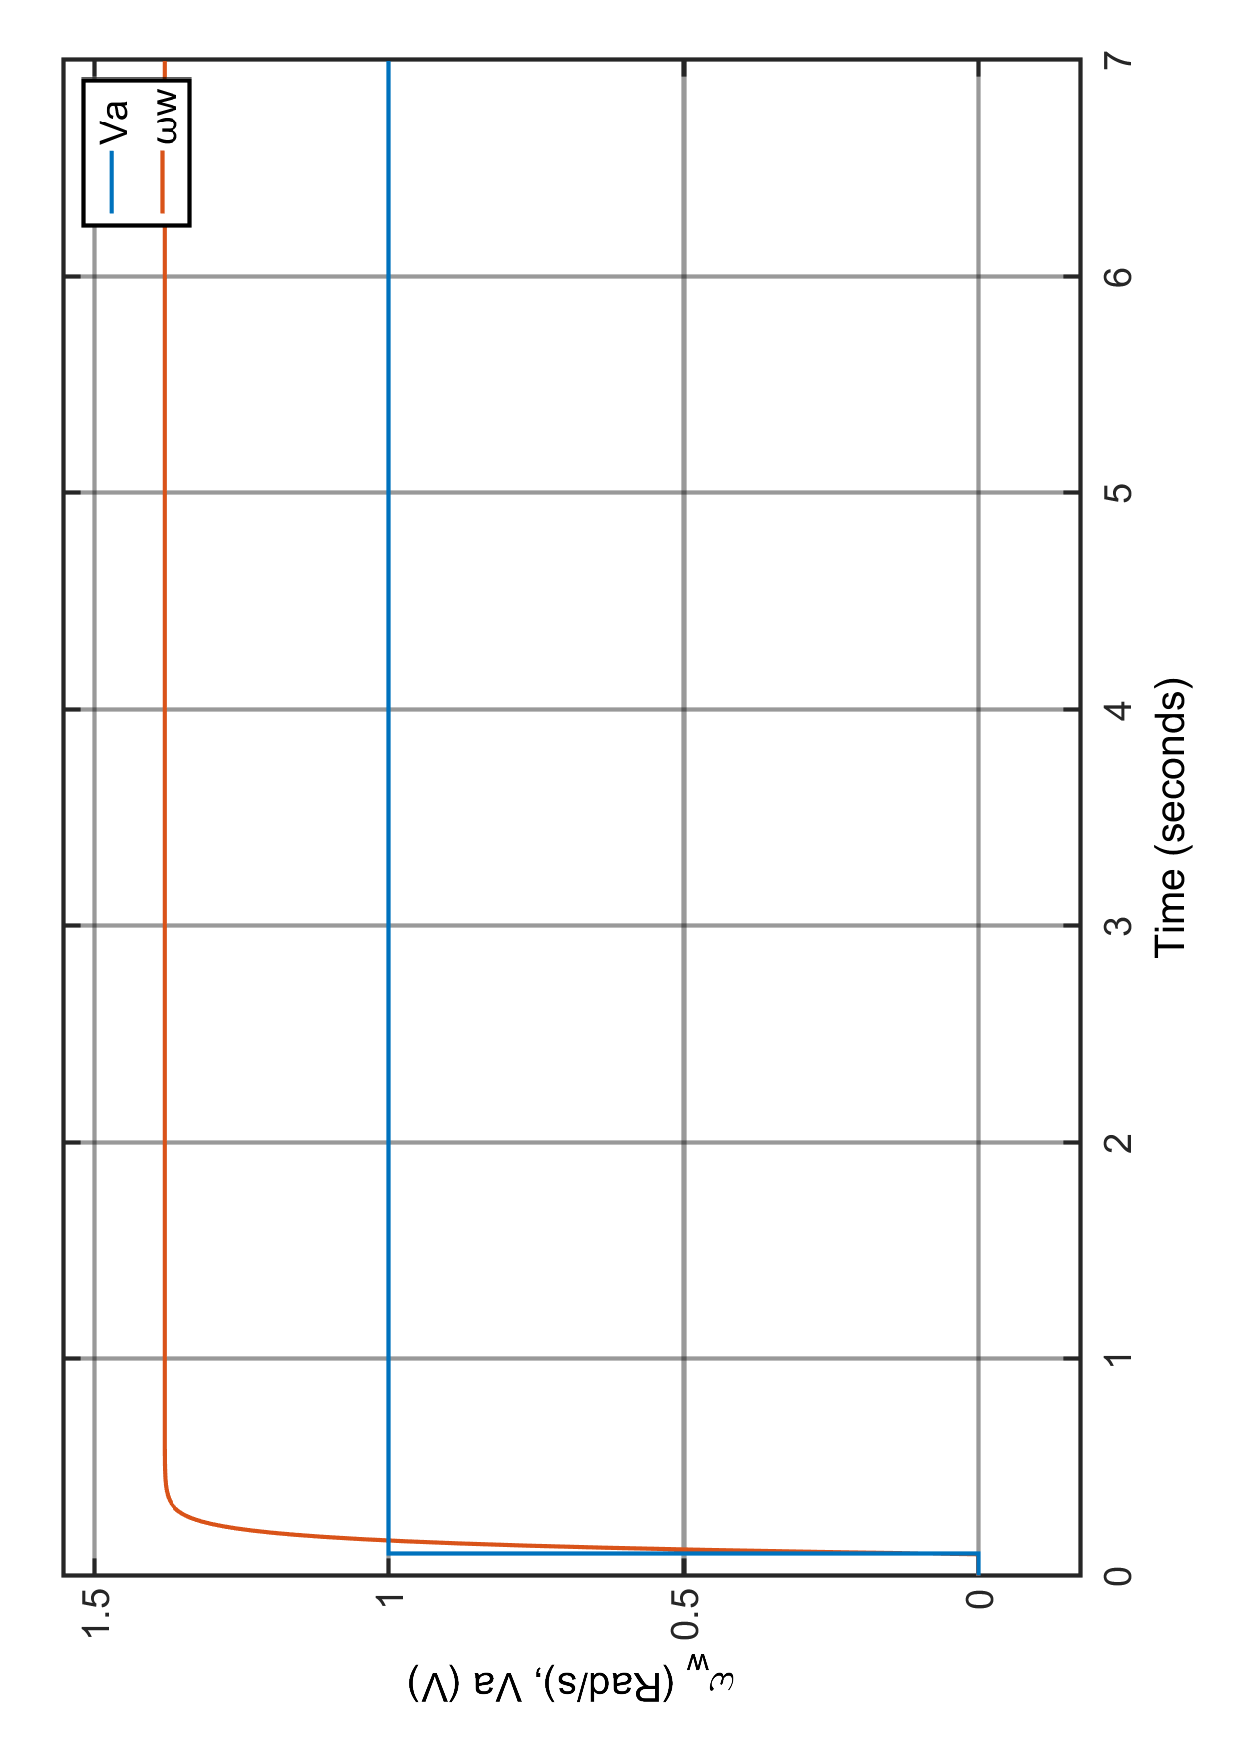
\includegraphics[height = 0.75\textwidth, angle = -90]{figures/motor1.pdf}
\caption{Simulation of motors and wheels model with an applied step as input.}
\label{fig:motor1}
\end{figure}
Looking at the expression for the motors and wheels model in \autoref{motorsAndWheels}, it is seen that the system is a first order when removing the final term in the expression. This is because the highest order of derivatives of $\omega_m(t)$ is one, giving a first order transfer function. This is partly due to the approximation done in \autoref{eq:electricMotor2} about disregarding the inductance in the motor.
From \autoref{fig:motor1}, it can be seen that the output of the motor mimics a first order system's output, as the response is approaching the reference, without any oscillation or overshoot, which is not possible for a first order system. Therefore, the output of the simulation matches what is expected, and the model is therefore assumed to be valid.

The inverted pendulum model \autoref{eq:model1W} is also simulated in Simulink. The input to this model is chosen to be $\ddot{x}_c$ since this is the input parameter in \autoref{eq:model1W}, by means of the expression $\ddot{x}_c = r_w\ddot{\theta}_w$. Also note that the inverted pendulum is initialised at an angle of -0.05 rad. The result can be seen in \autoref{fig:pend1}.
\begin{figure}[H]
\centering
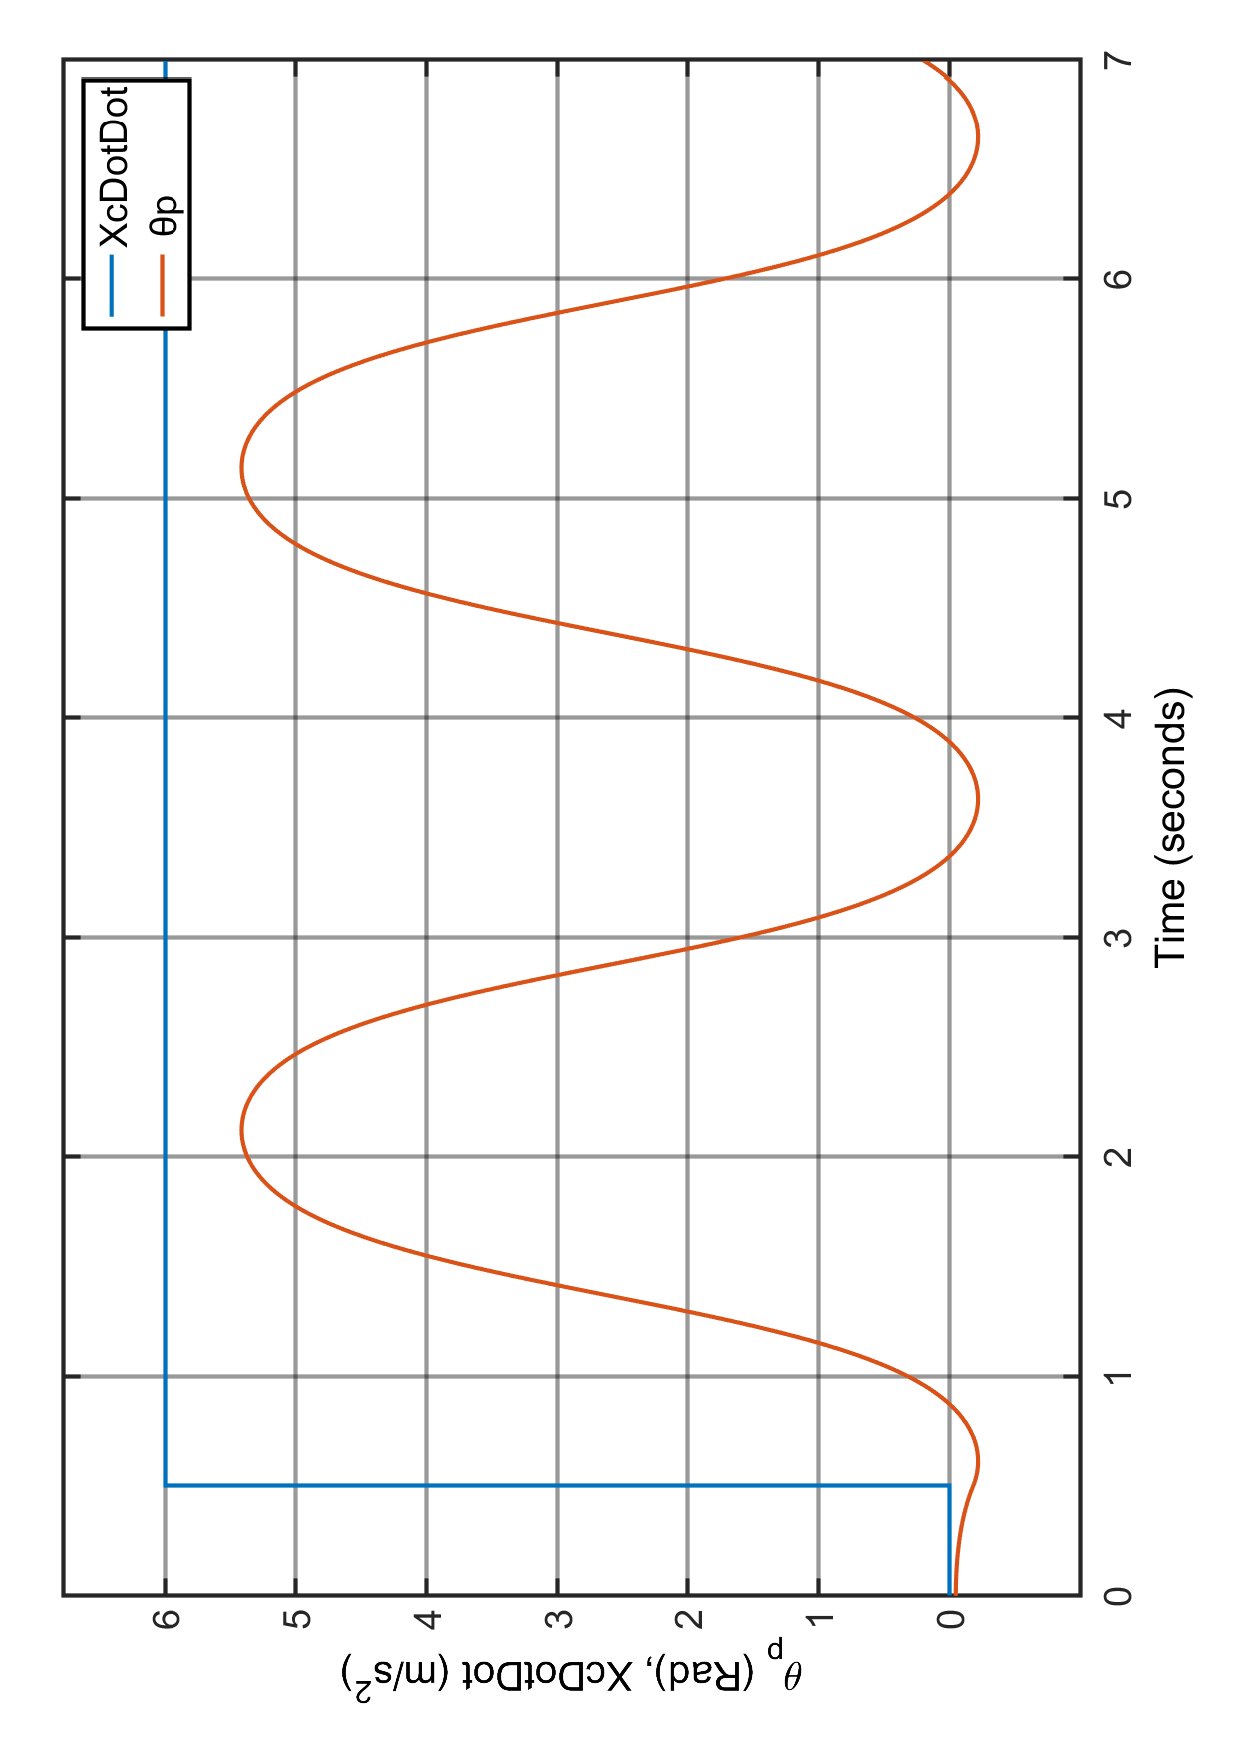
\includegraphics[height = 0.75\textwidth, angle = -90]{figures/pend1.pdf}
\caption{Simulation of the inverted pendulum model with an applied step as input.}
\label{fig:pend1}
\end{figure}

From \autoref{fig:pend1} it can be seen that the inverted pendulum starts tilting to one side, and when the step is applied, the angle changes direction and lastly the inverted pendulum oscillates around a certain angle. This angle is $\pi$ if the pendulum is swinging freely, corresponding to it hanging downwards, however an offset from $\pi$ is seen, due to the step applied. Thus, the inverted pendulum model is assumed to be valid.

To validate the system model, the motors and wheels model and the inverted pendulum model are combine and simulated in MATLAB. As an initial conditions for the simulation, the inverted pendulum is set at an angle of 1 radian, as this will cause the inverted pendulum to fall. Furthermore, a small friction is inserted in the inverted pendulum model to make the result comply more with expectations. This is done because the angle's magnitude otherwise grows, i.e. the inverted pendulum will oscillate more violently over time. This can be due to a sign error on a small number in the model. Time constraints prohibits the localisation and correction of this minor issue. The results of the simulation can be seen in \autoref{fig:systemVerification}.

\begin{figure}[H]
\centering
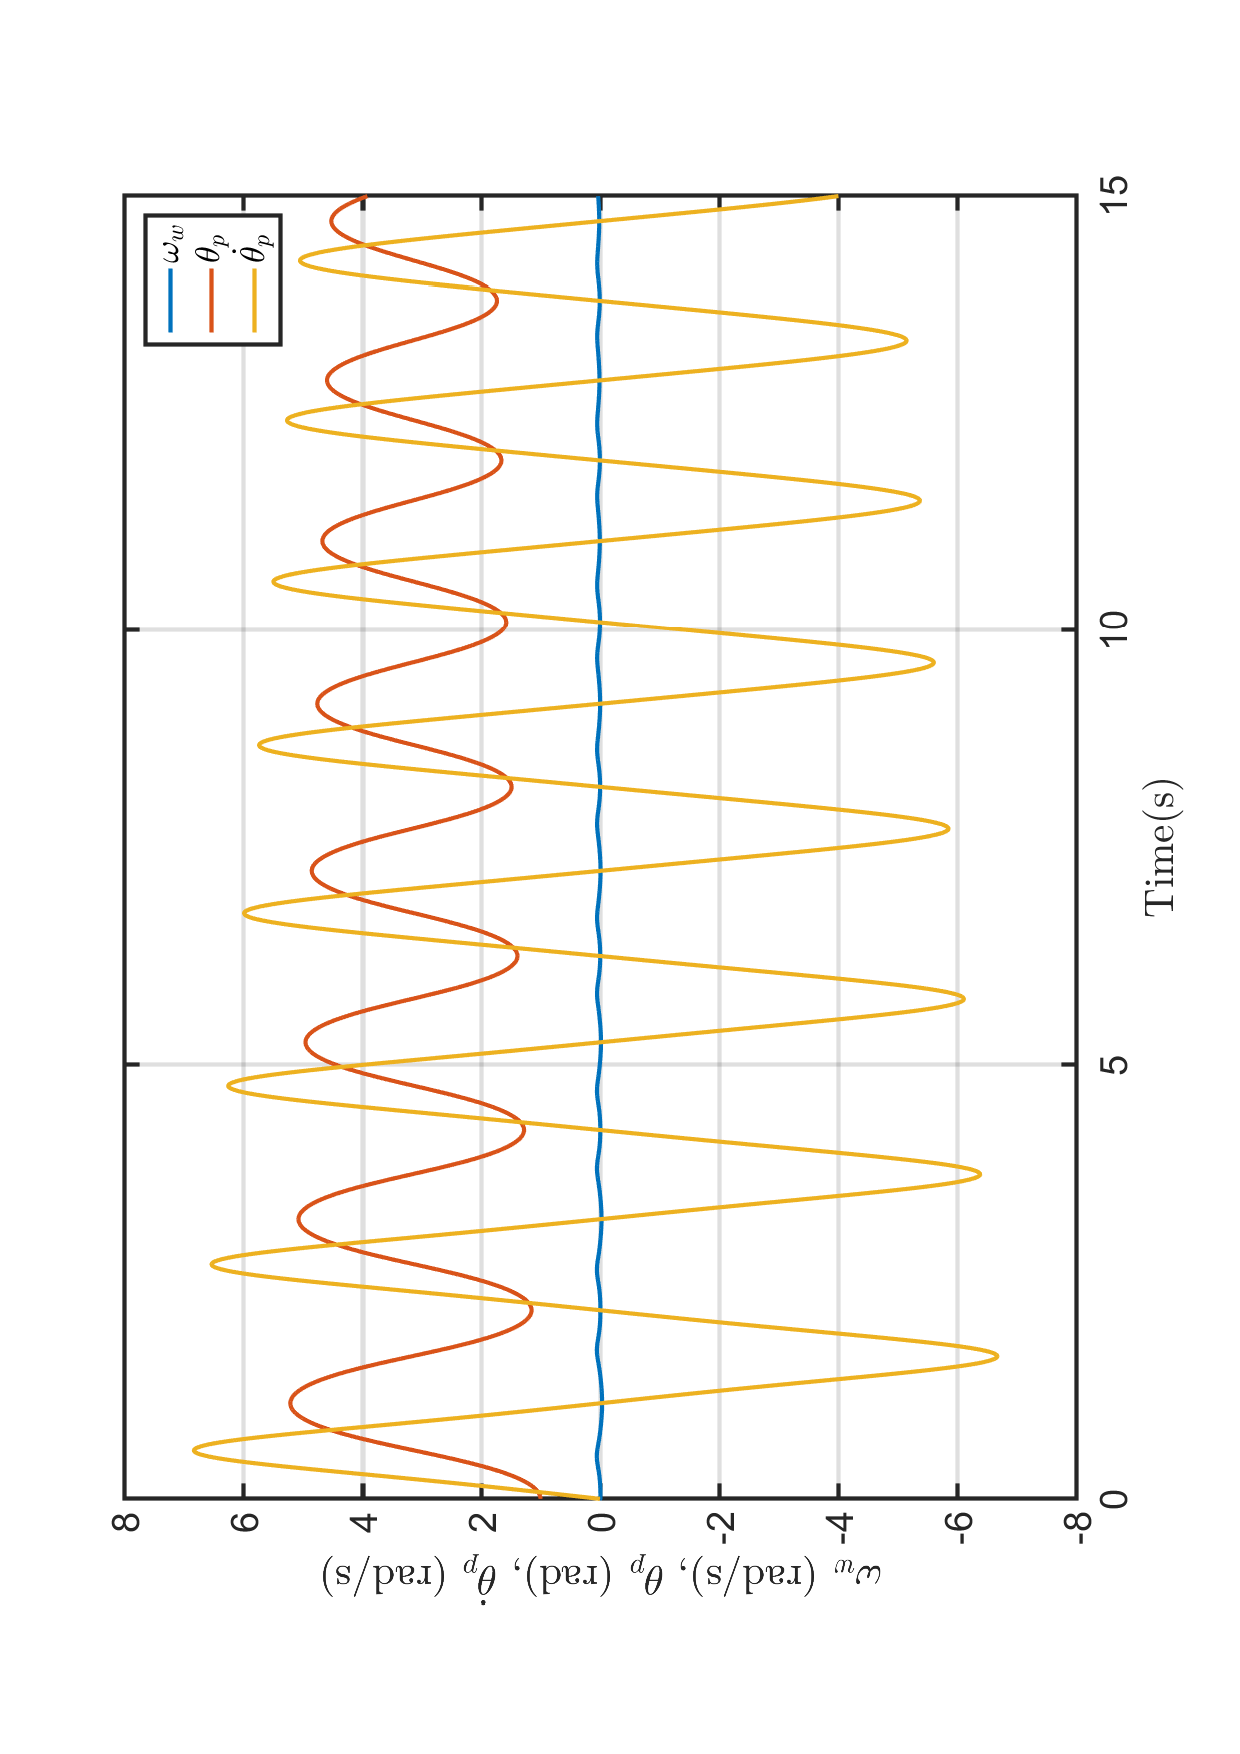
\includegraphics[height = 0.85\textwidth, angle = -90]{systemVerification.pdf}
\caption{Simulation of the system model by setting the inverted pendulum at 1 radian and no input. Note: a small friction is inserted in the model to comply more with expectations.}
\label{fig:systemVerification}
\end{figure}

From \autoref{fig:systemVerification}, it can be seen that the pendulum slowly loses magnitude due to the inserted friction. Also, it oscillates around $\pi$ which is to be expected. The model is hereby validated and can now be linearised.


\subsection{Linearisation of Derived Equations of Motion\label{subsec:Linearization}}
%In this section a transfer function describing the system is derived. This is done based on the three model equations, describing the behaviour of the segway. The transfer function is derived, so that it can be used when designing the controller. 
Before a transfer function of the system can be derived, it is necessary to linearise the two model equations, \autoref{eq:model1W} and \ref{motorsAndWheels}, as it is only linear equations that can be Laplace-transformed to form a transfer function.

It is seen that the only part of the motors and wheels model, \autoref{motorsAndWheels}, that is non-linear comes from \autoref{eq:model2W}, thus only this part needs to be linearised.
The second model equation, \autoref{eq:model1W}, also needs to be linearised as it contains non-linear terms. 

The method for doing the linearisation is chosen to be Taylor expansion.
%The last term in \autoref{motorsAndWheels} is the load torque $\tau_L$ \todo{why?}, and is approximately zero near the segway's operating point \todo{why?}. Thus \autoref{eq:motorsAndWheels} can be approximated as:
%\begin{equation}
%m_c \cdot r_w \cdot \ddot \theta_w(t) = 2 \cdot \frac{\Big(\frac{K_t}{R_A} \left( V_a(t) - K_e \cdot \frac{1}{N_{ms} N_{sw}} \cdot \dot\theta_w(t) \right) - \frac{1}{N_{ms} N_{sw}} \cdot \ddot\theta_w(t)J_{T} - \frac{1}{N_{ms} N_{sw}} \cdot \dot\theta_w(t) \cdot B_{T}\Big)}{r_w \cdot N_{ms} N_{sw}} \label{eq:model2S}
%\end{equation} 
%This approximation does not only simplify the expression considerably, but it also makes it a linear equation, as the load torque is the only nonlinear term in \autoref{eq:motorsAndWheels}.
%When approximating the load torque, it should be noted that it is only valid when the segway is at its operating point or very close to it. As the linearisation of the last model expression, \autoref{eq:model1W}, will be in the operating point as well, does not reduce the validity of the linearised model.\\
When linearising an equation, an expression for the tangent to the operating point is derived. 
% however is not alarming as the linearization of the other models, will be done in the equillibrium point as well.
%will be an approximation based on an operating point, which is in the segways equillibium position.\newpar
%The linearised model is the tangent to the chosen operating point. 
This is shown in \autoref{fig:taylor}. %This approach means that the linearised model is only an approximation of the original model around the operating point.
%During the course Modelling and control, the group was introduced to Taylor expansion as a method to linearise. For this reason the method that will be used to linearise \autoref{eq:model1W} is Taylor expansion.
\begin{figure}[H]
\centering
\input{figures/taylorFigure.ralf}
\caption{Illustration of linearisation principle.}
\label{fig:taylor}
\end{figure}

Taylor expansion is based on the Taylor series, shown in \autoref{eq:taylorSeries} \citep{sou:taylorSeries}. The Taylor series approximation of a signal is enhanced by including a greater number of terms in the Taylor series, i.e. by having an infinite sum of terms, the approximation is exact. However, since the linearisation is a tangent, only the first two terms in the Taylor series is used in the Taylor expansion, as the resulting expression is otherwise not linear.
\begin{align}
T(x) = f(a) + f'(a)(x - a) + \frac{f''(a)}{2!}(x - a)^2 + \frac{f^{(3)}(a)}{3!}(x - a)^3 + ...
\label{eq:taylorSeries}
\end{align}
\begin{where}
\begin{tabular}{p{40pt} p{42pt} p{200pt}} &$T$ & is the taylor approximation \end{tabular} \\
\begin{tabular}{p{40pt} p{42pt} p{200pt}} &$x$ & is the input \end{tabular} \\
\begin{tabular}{p{40pt} p{42pt} p{200pt}} &$f$ & is the function to be linearised \end{tabular} \\
\begin{tabular}{p{40pt} p{42pt} p{200pt}} &$a$ & is the linearisation point \end{tabular} \\
\end{where}

The linearisation is performed around the segway's operating point, which is expressed as:
\begin{equation}
\theta_p(t) = \bar{\theta}_p(t) + \hat{\theta}_p(t)
\end{equation}
\begin{where}
\va{$\theta_p(t)$}{is the angle of the inverted pendulum}{rad}\\
\va{$\bar{\theta}_p(t)$}{is the operating point}{rad}\\
\va{$\hat{\theta}_p(t)$}{is the deviation from the operating point}{rad}
\end{where}

There are three variables included in the non-linear terms in the equations that are to be linearised, i.e. $\theta_p(t)$, $\dot\theta_p(t)$ and $\ddot\theta_p(t)$. Therefore, the Taylor series has to be done for each variable, which can then be added to form the linear expression with multiple linearised variables. The Taylor expansion can be expressed as the following:
\begin{align}
T= f(\bar{\theta}_p(t),\bar{\dot \theta}_p(t), \bar{\ddot \theta}_p(t))+ \frac{\partial f(\bar{\theta}_p(t))}{\partial\theta_p(t)}\cdot \hat{\theta}_p(t)+\frac{\partial f(\bar{\dot \theta}_p(t))}{\partial \dot \theta(t)_p}\cdot \hat{\dot \theta}_p(t) &+ \frac{\partial f(\bar{\ddot \theta}_p(t))}{\partial \ddot \theta(t)_p}\cdot \hat{\ddot \theta}_p(t)\label{eq:taylor}
\end{align}

The linearisation is done in the segway's upright position $\theta_p = 0$, i.e. this is the chosen operating point.

First, the cart model, \autoref{eq:model2W}, is linearised. This is done in \appref{appTaylor}, and the result can be seen in \autoref{linGovEq2}.
\begin{equation}
(m_c + m_p) \cdot \ddot x_c(t) = F_{F}(t) + m_p \cdot l \cdot \hat{\ddot{\theta}}_p(t)\label{linGovEq2}
\end{equation}

Analysing this equation, and comparing it to \autoref{fig:systemVerification}, it is assumed that when the segway is being operated, i.e. a voltage is applied to the motors and the segway is therefore moving, the following is true:
$$ F_F(t) >> m_p \cdot l \cdot \hat{\ddot{\theta}}_p(t) $$
This means that the force applied from the motors is much bigger than the force the inverted pendulum exerts on the cart. Based on this assumption, the inverted pendulum's influence on the cart's position is neglected, i.e. the last term in \autoref{linGovEq2} is removed. In a physical sense, this would mean that when the inverted pendulum is tilting, the cart will not move. Obviously, this is not the case, but the movement caused by the inverted pendulum is much smaller than the movement caused by the motors and wheels, and it is therefore seen as a fair assumption to make. This serves to make the model simpler, by removing the feedback from the pendulum to the cart.\\
This simplified linearised expression can then be combined with \autoref{eq:model3W} and \autoref{eq:tauFFrelation}, to obtain a linear expression for the motors and wheels model, which can be seen in \autoref{eq:model2S}.
\begin{equation}
(m_c + m_p) \cdot r_w \cdot \ddot \theta_w(t) = 2 \cdot \frac{\Big(\frac{K_t}{R_a} \left( V_a(t) - \frac{K_e}{N_{ms} N_{sw}} \cdot \dot\theta_w(t) \right) - \frac{J_{T}}{N_{ms} N_{sw}} \cdot \ddot\theta_w(t) - \frac{B_{T}}{N_{ms} N_{sw}} \cdot \dot\theta_w(t) \Big)}{r_w \cdot N_{ms} N_{sw}} \label{eq:model2S}
\end{equation} 

With the motors and wheels model linearised, the inverted pendulum model shall also be linearised. The inverted pendulum model, see \autoref{eq:model1W}, is linearised in \appref{appTaylor}, which yields:
\begin{align}
(J_p+m_p\cdot l^2)\cdot \hat{\ddot \theta}_p(t) = m_p \cdot l \Big(g \cdot \hat{\theta}_p(t) + r_w \cdot \ddot \theta_w(t)   
\Big)\label{eq:firstModelLin}
\end{align}
Both model expressions are now linear and can be Laplace transformed to yield transfer functions, which is necessary to be able to design a controller for the segway. The segway's transfer function is now to be determined.
%The equation are shown in \autoref{eq:firstModel}, where each term that will be linearised by applying the Taylor expansion, shown in \autoref{eq:taylor}, is marked. The linearised approximation is shown in \autoref{eq:firstModelLin}.



%\subsection{Laplace Transform}
From the previous sections tree expressions have been derived. One for the motor model and one for the pendulum model. Moreover an expression, which is the link between the two models, is found. 
The motor model is the following:
\begin{equation}
\tau_a(t) = \frac{k_t}{R_A} \left( V_a(t) - K_e \cdot \dot\theta_m(t) \right) - \ddot\theta_m(t)J_{T} - \dot\theta_m(t)B_{T}  \label{eq:motorfinal2}
\end{equation}
Laplace transforming \autoref{eq:motorfinal2} yields:
\begin{align}
\tau_a(s)&=\frac{k_t}{R_A}- \Theta_m(s) (s\cdot \frac{k_t+k_e}{R_a}+s\cdot B_T+s^2\cdot J_T)\\
&=\frac{k_t}{R_A}- \Theta_m(s)(s^2\cdot J_T+s(\frac{k_t+k_e}{R_a}+B_T))
\end{align}
The link between the two models shall be laplace transformed as well. The link in time domain is:
\begin{align}
 \hat{\ddot\theta}_m(t)=\frac{(J_p+m_p\cdot l^2)\hat{\ddot \theta}_p(t)}{m_p\cdot l\cdot r_w\cdot N_{ms}\cdot N_{sw}}-\frac{g\cdot \hat{\theta}_p(t)}{r_w\cdot N_{ms}\cdot N_{sw}}\label{eq:linktime}
\end{align}
Laplace transforming \autoref{eq:linktime} yields:
\begin{align}
s^2\cdot \Theta_m(s)&= \frac{(J_p+m_p\cdot l^2)s^2\cdot \Theta_p(s)}{m_p\cdot l \cdot r_w \cdot N_{ms}\cdot N_{sw}}-\frac{g\cdot \Theta_p(s)}{r_w\cdot N_{ms}\cdot N_{sw}}\\
\Rightarrow \Theta_m(s)&= \frac{(J_p+m_p\cdot l^2)\Theta_p(s)}{m_p\cdot l \cdot r_w \cdot N_{ms}\cdot N_{sw}}-\frac{g\cdot \Theta_p(s)}{s^2 \cdot r_w\cdot N_{ms}\cdot N_{sw}}
\end{align}
Lastly the model for the pendulum. The model expression is: 
\begin{equation}
(J_p+m_p\cdot l^2)\hat{\ddot \theta}_p(t)(m_p+m_c)=(m_p^2+m_c)l\cdot g \cdot \hat{\theta}_p(t)+m_p^2\cdot l^2 \cdot  \hat{\ddot\theta}_p(t)+2\cdot F_F(\theta_p(t))\label{eq:penmodel11}
\end{equation}
Laplace transforming \autoref{eq:penmodel11} yields:
\begin{equation}
s^2(J_p+m_p\cdot l^2)\Theta_p(s)(m_p+m_c)=(m_p^2+m_c)l\cdot g \cdot \Theta_p(s) + m_p^2 \cdot l^2 \cdot s^2\cdot \Theta_p(s) +2\cdot F_F(\Theta_p(s))
\end{equation}
As the input to pendulum from the motors are the applied force, it is preferable to have this linearized model as an expression of the applied force. 
\begin{equation}
2\cdot F_F(\Theta_p(s))=\Theta_p(s)(s^2((J_p+m_p\cdot l^2)(m_p+m_c)-m_p^2\cdot l^2)-(m_p^2 + m_c)l\cdot g)
\end{equation}

%
%\begin{align}
%&s^2\cdot \theta\cdot (l\cdot (m_p+m_c-m_p))-\theta \cdot g(m_p+m_c)=F_F\nonumber\\
%&\Rightarrow \frac{\theta}{F_F}=\frac{1}{s^2\cdot (l\cdot (m_p+m_c)-g(m_p+m_c)}\nonumber \\
%&\Rightarrow \frac{\frac{1}{l\cdot m_c}}{s^2-\frac{g(m_p+m_c}{l\cdot m_c}}
%\end{align}
%It shows, that the transfer function is the same as the one derived at with the taylor expansion approximation. \\
%The linear approximation of the inverted pendulum model is therefore assumed valid. 
%
%
%
%%\Rightarrow\frac{2.377}{s^2 - 37.369}
%%\Rightarrow \theta(s)\cdot s^2\cdot l ((m_p+m_c)-m_p)=g\cdot \theta(s)\cdot (m_p+m_c)+F_F(s)\nonumber\\
%%\Rightarrow \theta(s)\cdot s^2\cdot l(m_p+m_c-m_p)-g\cdot \theta(s)\cdot(m_p+m_c)=F_F(t)\nonumber\\
%%\Rightarrow \theta(s)\cdot (s^2\cdot l \cdot (m_p+m_c))=F_F(t) \nonumber \\
%The transfer function for the inverted pendulum shall be merged with a transfer function for the motors and wheels model to allow design and implementation of a controller. Merging the transfer functions is done in the following section. 

%\section{Merging of models}
From the previous section three linearized expressions can be extracted. These are ow to be combinded such that a final expression is derived, representing the entire system.
The expressions are as follows:

\begin{align}
\tau_a(s)&=\frac{K_t}{R_A}- \Theta_m(s)\cdot(s^2\cdot J_T+s(\frac{k_t+k_e}{R_a}+B_T))\label{eq:1}\\
\Theta_m(s)&= \frac{(J_p+m_p\cdot l^2)s^2\cdot \Theta_p(s)}{m_p\cdot l \cdot r_w \cdot N_{ms}\cdot N_{sw}}-\frac{g\cdot \Theta_p(s)}{s^2 \cdot r_w\cdot N_{ms}\cdot N_{sw}} \label{eq:2}\\
2\cdot F_F(\Theta_p(s))&=\Theta_p(s)(s^2(J_p+m_p\cdot l^2)(m_p+m_c)-m_p^2\cdot l^2)-(m_p^2 + m_c)l\cdot g \label{eq:3}
\end{align}

Combining \author{eq:1} and \autoref{eq:2} yields:
\begin{equation}
F_F(\Theta_p(s))=\frac{\frac{k_t}{R_a}\cdot V_a-(\frac{(J_p+m_p\cdot l^2)\Theta_p(s)}{m_p\cdot l\cdot r_w \cdot N_{ms}\cdot N_{sw}}-\frac{g\cdot \Theta_p(s)}{s^2\cdot r_w \cdot N_{ms}\cdot N_{sw}})(s^2\cdot J_t+s(\frac{k_t\cdot k_e}{R_a}+B_T))}{r_w} \label{eq:4}
\end{equation}
Note that the applied force $F_F(\Theta_p(s))$ is eual to the torque $\tau_a(s)$ when multiplied with the wheel ratio $r_w$, as torque is the product of force and length. \newpar
Now the motor model is combined  with the link-expression. This allows to connect all three equations. This is done by inserting \autoref{eq:4} into \autoref{eq:3}.
\begin{align}
(\Theta_p(s)(s^2(J_p+m_p\cdot l^2)(m_p+m_c)-&m_p^2\cdot l^2)-(m_p^2 + m_c)l\cdot g )\cdot r_w  \\ \nonumber
=\frac{k_t}{R_a}\cdot V_a-(\frac{(J_p+m_p\cdot l^2)\Theta_p(s)}{m_p\cdot l\cdot r_w \cdot N_{ms}\cdot N_{sw}}-&\frac{g\cdot \Theta_p(s)}{s^2\cdot r_w \cdot N_{ms}\cdot N_{sw}})(s^2\cdot J_t+s(\frac{k_t\cdot k_e}{R_a}+B_T))
\end{align}

The deriviation of the transferfunction of the entire system is in the appendix \todo{ref}. The final expression is fairly large, why each term has been given a letter to represent it in the transfer function here.
\begin{equation}
\frac{\Theta_p}{V_a}=\frac{k_t\cdot s}{R_a(s^3\cdot A + s^2 \cdot B + s(C_D)-E)}
\end{equation}






The linear model for the motors and wheels system and the one for the inverted pendulum, are in this section merged to form the linear model for the segway. The linear model for the inverted pendulum is shown in \autoref{eq:invPenLin_Merge}, and the linear model for the motors and wheels are shown in \autoref{eq:motorWheel_Merge}.

\begin{equation}
\frac{F_F(s)}{V_a(s)} = \frac{0.049s}{0.040s + 1}
\label{eq:motorWheel_Merge}
\end{equation}

\begin{align}
\frac{\theta_p(s)}{F_F(s)}=\frac{\frac{1}{l\cdot m_c}}{s^2-\frac{g\cdot (m_p+m_c)}{l\cdot m_c}}=\frac{2.377}{s^2 - 37.369}
\label{eq:invPenLin_Merge}
\end{align}

To merge these transfer functions, with the purpose of achieving one transfer function with $V_a(s)$ as input and $\theta_p(s)$ as output. The two transfer functions, \autoref{eq:invPenLin_Merge} and \autoref{eq:motorWheel_Merge}, are multiplied, since the two transfer functions are in series as shown in \autoref{fig:modelOverall} and can therefore be multiplied to get the output. This yields the transfer function for the segway shown in \autoref{eq:segwayTf}.

\begin{align}
\frac{\theta_p(s)}{V_a(s)} &= \frac{2.9s}{s^3 + 25s^2 - 37.5s - 943.75} = \frac{2.9s}{(s + 25)(s + 6.15)(s - 6.14)}
\label{eq:segwayTf}
\end{align} 
Now that the combined transfer function has been determined, it needs to be verified through comparison with test results.

It is decided to remove the pole in -25, based on the impulse response, as it is seen that this pole does not have much influence. Thus, the system is reduced to a 2'nd order system, with a zero in zero.

This is put into matlab to do parameter estimation again.
We see that the gain is off by a factor of about 3 by looking at the input/output graphs of the measurements, so the gain is changed. This is thus the model we use as our guess for Matlab to estimate from.
\begin{figure}[H]
    \centering
    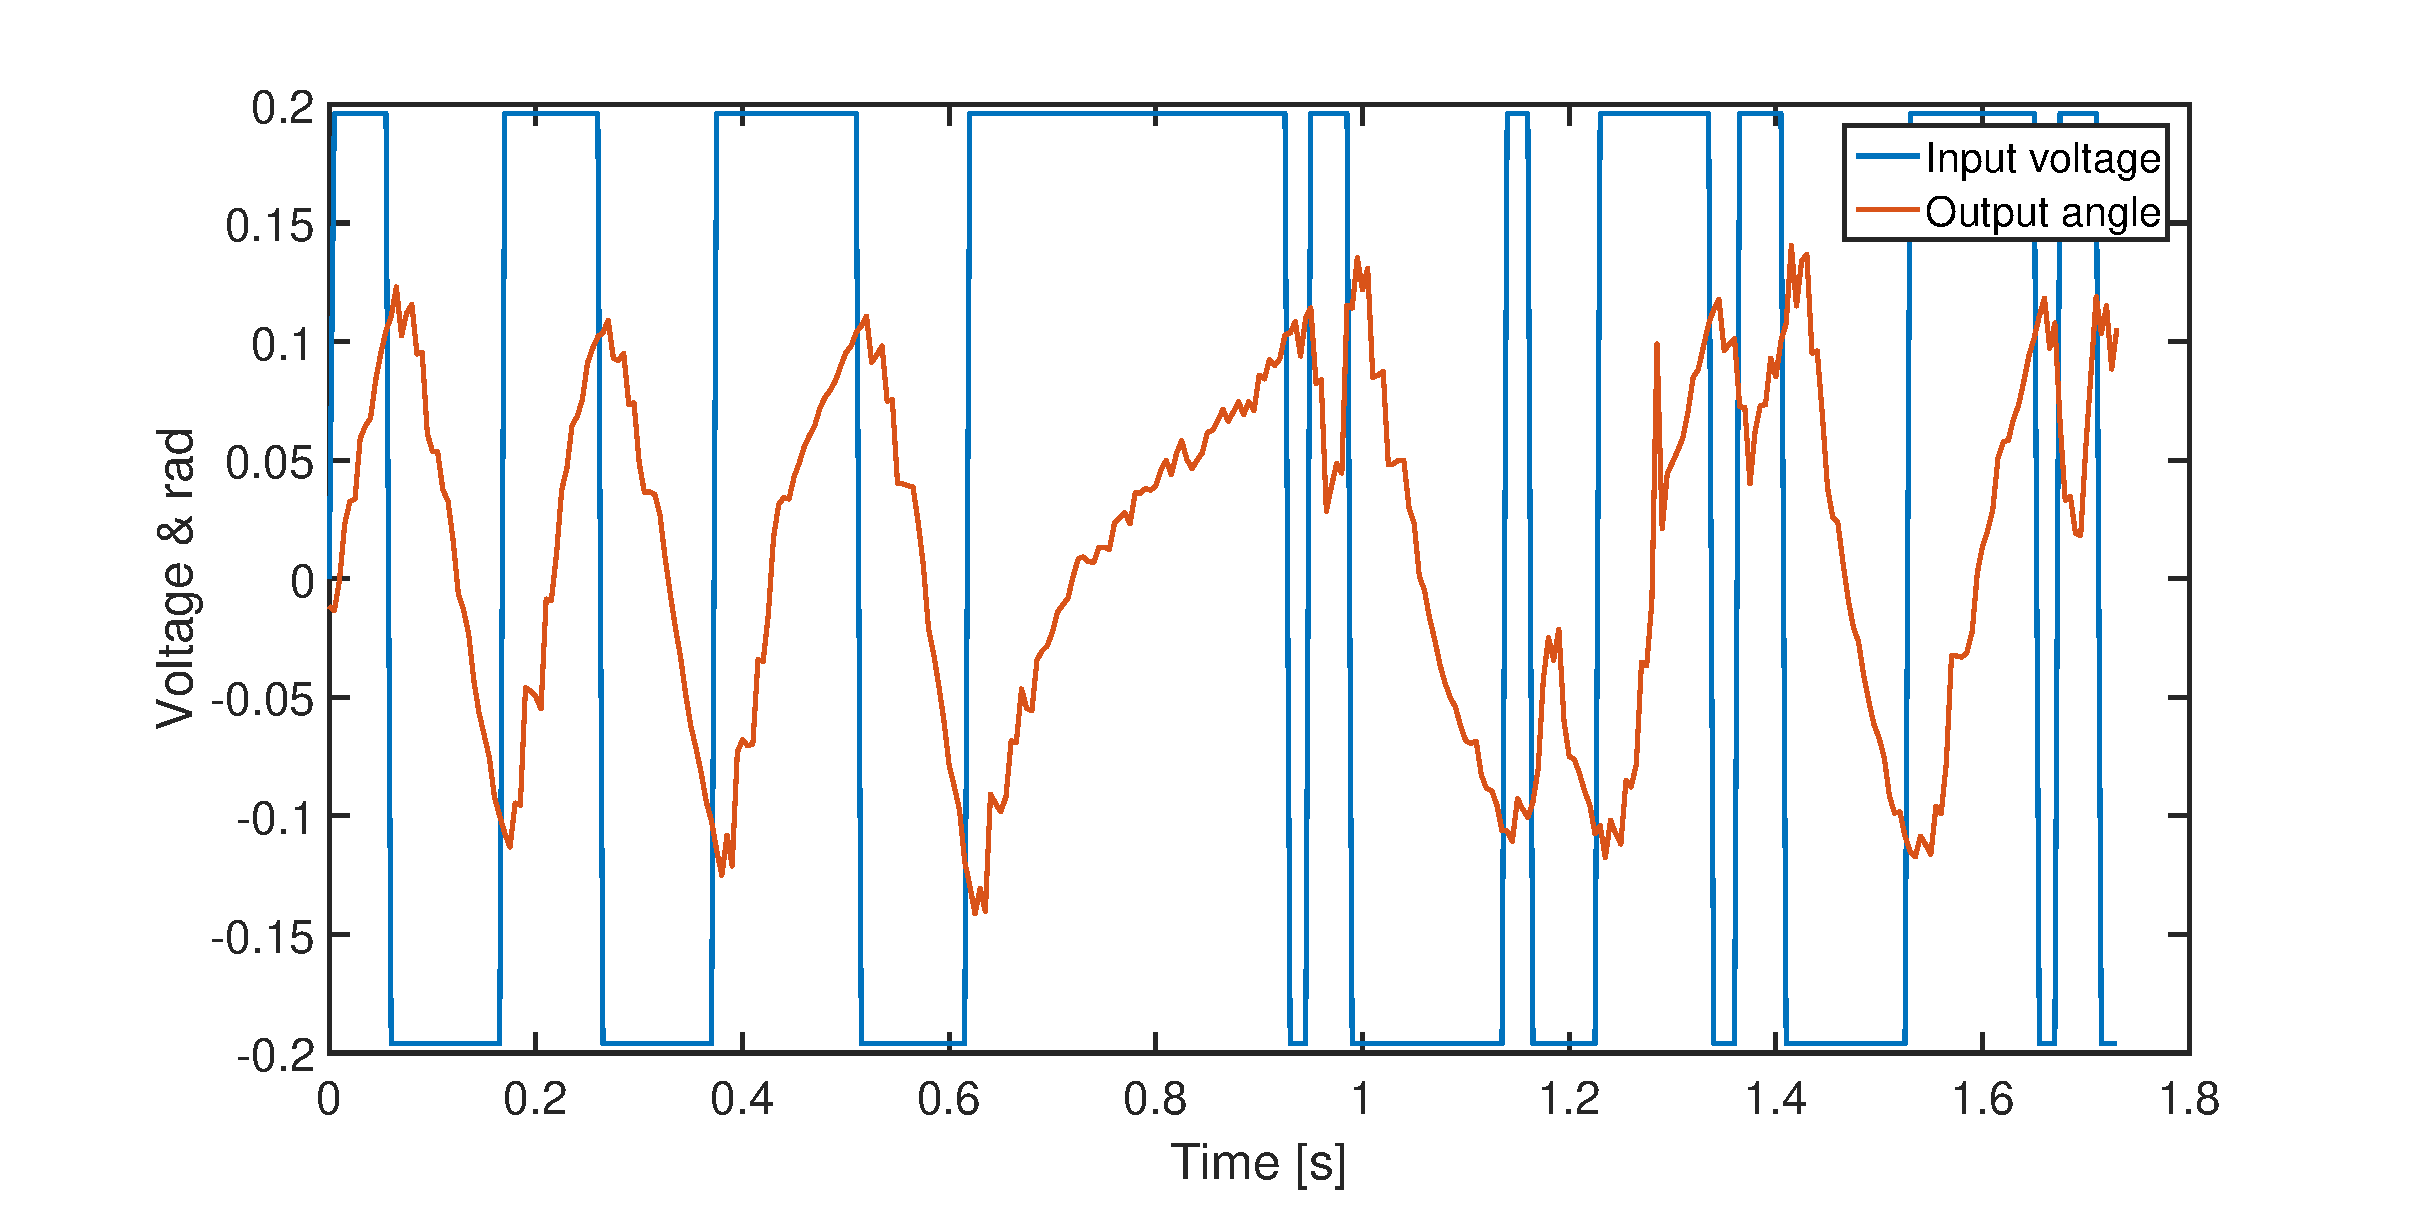
\includegraphics[width = \textwidth]{ParameterEstimationSegway.eps}
    \caption{Input voltage and output angle of segway for model verification.}
    \label{fig:paramEst3}
\end{figure} 


\begin{figure}[H]
    \centering
    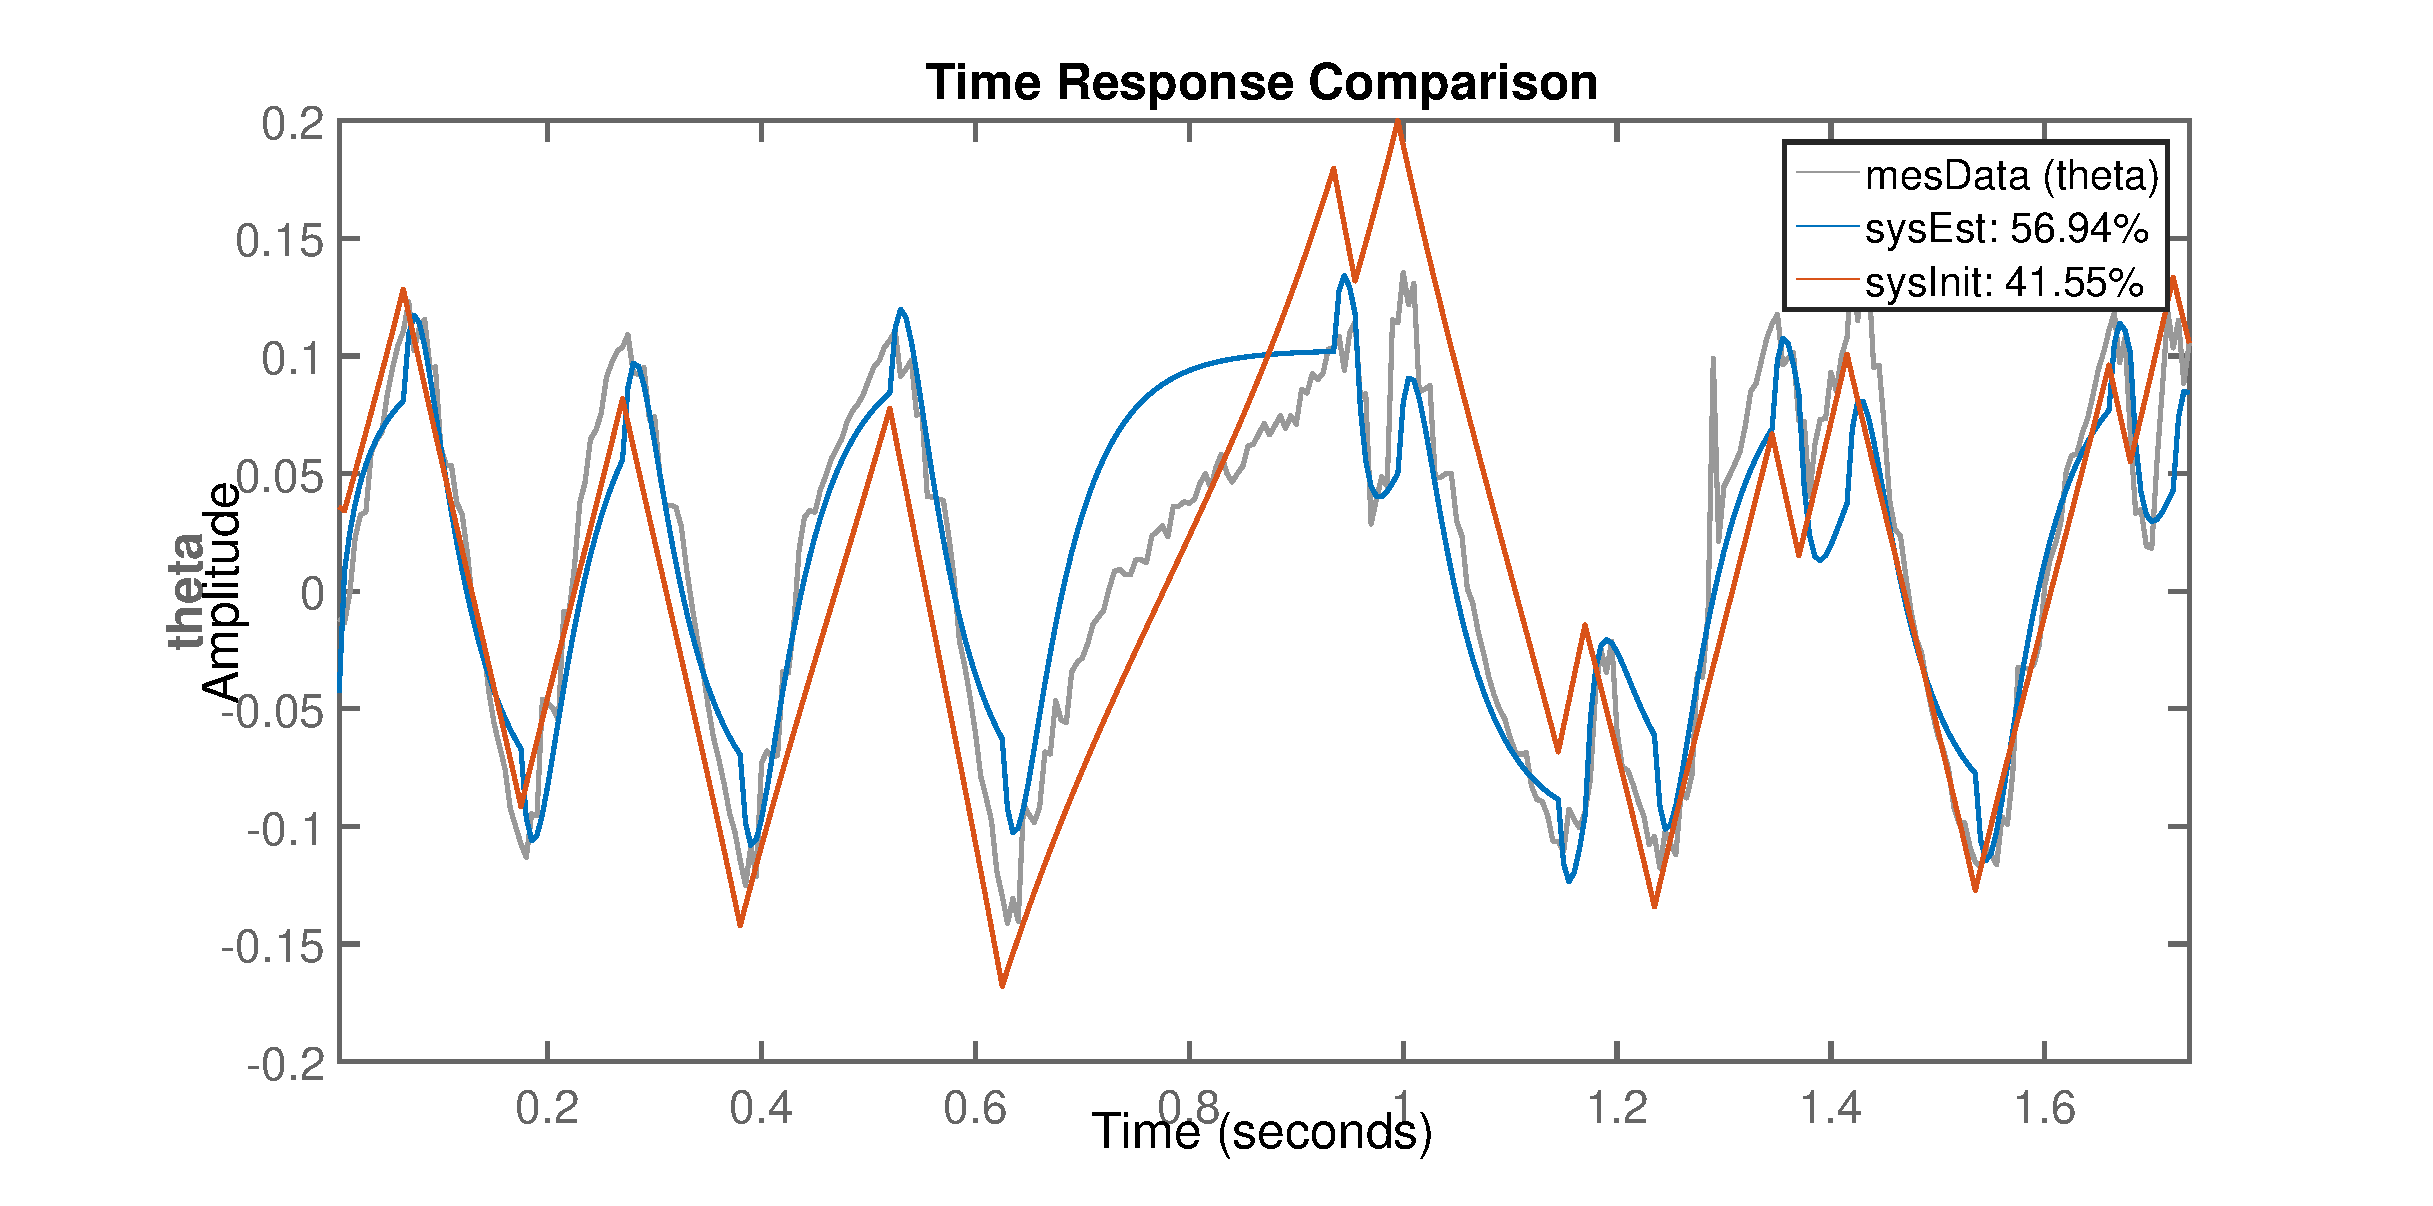
\includegraphics[width = \textwidth]{ParameterEstimationSegway2.eps}
    \caption{System initial guess, measurements and Matlab estimate.}
    \label{fig:paramEst4}
\end{figure} 

Matlab provides the following transfer function:

\begin{align}
\frac{\theta_p(s)}{V_a(s)} &= \frac{-2.015 s + 100.2}{s^2 + 112.3 s + 1918} = \frac{-2.015 (s - 49.7)}{(s + 91)(s + 21)}
\label{eq:wrongTF}
\end{align} 


%\subsection{Equations of motion}
-Why have a model \\
- what our model shall describe\\
- Aim of the chapter and the procedure\\


- open loop , what does it describe concerning our system\\
- closed loop, what does it describe concerning our system\\

Equations of motion, verifying model, linearization, verifying model\\
Compare to real life measurements\\
Approval of model\\
Block diagram and open and closed loop - analysis \\
Transferfunction and the different unit throughout the system\\
Step response, overshoot, peak time, settling time and steady state error\\
Bodeplot, phase and gain margins and how they affect the system\\
Combinning the two models\\
-\\
-\\
Design the controller in relation to model analysis\\
Simulation of model with controller\\
Test and adjustments\\

Implementation of controller\\
Test concerning requirements and analysis from vicon data\\\\\\\\


A mathematical model is designed to identify a systems dynamics with the purpose of analysis which shall lead to the design of a controller. A model  shall be as true to reality as needed for the specific control purpose.
The derived model will be nonlinear, as the world is nonlinear. The model will should be verified in relation to the real world, whereafter the model can be linearised. Linearisation of the model eases the design of an effective controller.\\\\%&Therefore it is necessary to make some assumptions. These assumptions will make the model more inaccurate, thus this should be done with careful consideration.
%Based on the system's model, the behaviour of the system can be analyzed and therefore controlled.\\
This section first derives the inverted pendulum dynamics expressed in the equations of motion, which is subsequently verified and afterwards linearized and a transferfunction will be derived. From the transferfunction the system's stability and behaviour can be extracted by analysis of the system's step response and bodeplots. 
\\\\
The model of the inverted pendulum shall describe how the two masses, the cart and the pendulum, behave when a force is exerted by the surroundings. Note that the rod is assumed massless, and will therefore not be modelled. The inverted pendulum is shown in\autoref{fig:mecmodinvpen}.
\begin{figure}[H]
\centering
\scalebox{3}{\input{figures/invpenmec.ralf}}
\caption{Mechanical model of the inverted pendulum.}
\label{fig:mecmodinvpen}
\end{figure}
In \autoref{fig:mecmodinvpen} the mass at the end of the rod is M1, the variable $\theta$ describes the angle of the pendulum/rod from a vertical line at the center of the cart. Note, that the angle is positive in the counterclockwise direction. This angle can be described in relation to both the y and x direction. The force $F_B$ is a friction force exerting upon the mass M2. The force applied to move the minisegway is labelled $F_F$. \\\\
From \autoref{fig:mecmodinvpen} free body diagrams can be determined. A free body diagram has the purpose to depict the forces acting upon an object. In this case the pendulum's free body diagrams is representing the forces acting upon the mass at the end of the pendulum and the cart while the minisegway is in a upright position. From the free body diagrams equations of motion can be derived, which shall lead to a transfer function that describes the system's behaviour.\\
The free body diagram of the mass at the end of the assumed massless rod is shown in \autoref{fig:fbdm1}.
\begin{figure}[H]
\centering
\scalebox{0.9}{\input{figures/invpen_M1_FBD.ralf}}
\caption{Free body diagram of the mass at the end of the massless rod.}
\label{fig:fbdm1}
\end{figure}
The forces exerted on the the mass, M1, is the gravitationalforce, $F_g$. The force $F_t$ is the tension in the rod between the pendulum and the cart. The magnitude of this force depends on the angle, $\theta$.\\\\
The free body diagram of the mini segways cart is shown in \autoref{fig:fbdm2}.
\begin{figure}[H]
\centering
\scalebox{1.3}{\input{figures/invpen_M2_FBD.ralf}}
\caption{Free body diagram of the cart.}
\label{fig:fbdm2}
\end{figure}
\autoref{fig:fbdm2} shows the free body diagram of the mini segways cart. The force $F_g$ is the gravitational force and $F_N$ is the force pushing upwards from the ground. The force $F_B$ is the force acting in the opposite direction of the applied force $F_F$ due to friction. The force $F_t$ is the tension of the rod between the pendulum and the cart. Note that its magnitude is equal to the force acting upon the pendulum, but opposite in direction. The angle $\theta$ determines the magnitude of the force $F_t$.



%\begin{figure}
%\centering
%\input{Report/figures/invpenmec.ralf}
%\caption{Inverted pendulum.} \label{fig:pen_mek_overview}
%\end{figure}
%
%\begin{figure}
%\centering
%\input{Report/figures/invpen_M1_FBD.ralf}
%\caption{Free body diagram for the mass at the pendulum.} \label{fig:fbdm1}
%\end{figure}
%
%\begin{figure}
%\centering
%\input{Report/figures/invpen_M2_FBD.ralf}
%\caption{Free body diagram for cart.} \label{fig:fbdm2}
%\end{figure}
From the free body diagrams it is now possible to express the dynamics of these in equations of motion. \\\\
For the pendulum:
\begin{align}
m_1 \cdot \ddot x_1 &= F_t \cdot \sin(\theta) \label{eom1}\\
m_1 \cdot \ddot y_1 &= -F_g -F_t \cdot \cos(\theta) \label{eom2}
\end{align}
For the chart:
\begin{align}
m_2 \cdot \ddot x_2 = -B\cdot \dot x_2 - F_t \cdot \sin(\theta)+F_F \label{eom3}
\end{align}
Kinematics:
\begin{align}
\vv{a_1} = L\cdot \ddot \theta\cdot \vv{\epsilon_\theta} + L \cdot \dot \theta ^2 \cdot \vv{\epsilon_r} + \ddot x_2 = \vv{a_{1/2}}+\vv{a_2} \label{eom4}
\end{align}
\begin{align}
\ddot x_1&=\vv{a_{x1}}= -L \cdot \ddot\theta\cdot \cos(\theta) + L \cdot \dot \theta^2 \cdot \sin(\theta)+\ddot x_2  \label{eom5} \\
\ddot y_1&=\vv{a_{1y}}=-L\cdot \ddot\theta\cdot\sin(\theta) - L \cdot \dot \theta^2 \cos(\theta)\label{eom6}
\end{align}
----------\\

\autoref{eom5} into \autoref{eom1}:
\begin{align}
-m_1\cdot L\cdot \ddot \theta \cdot \cos(\theta)+m_1 \cdot L\cdot \dot \theta^2 \cdot \sin(\theta)+m_1\cdot \ddot x_2 = F_t \cdot \sin(\theta) \label{eom7}
\end{align}
\autoref{eom6} into \autoref{eom2}:
\begin{align}
-m_1 \cdot L \cdot \ddot \theta\cdot\sin(\theta) - m_1 \cdot L\cdot \dot \theta^2\cdot \cos(\theta)=-m_1\cdot g - F_t \cdot \cos(\theta)\label{eom8}
\end{align}
%Multiply with $\cos(\theta)$ on both sides in  \autoref{eom7}:
%\begin{align}
%-m_1\cdot L \cdot \ddot \theta \cdot \cos^2 (\theta)+m_1\cdot L \cdot \dot \theta^2 \cdot \sin(\theta)\cdot \cos(\theta)+m_1\cdot \ddot x_2 \cdot \cos(\theta)=F_t\cdot \cos(\theta)\cdot \sin(\theta)\label{eom9}
%\end{align}
%Multiplying with sine on both $\sin(\theta)$ in \autoref{eom8}:
%\begin{align}
%-m_1\cdot L\cdot \ddot \theta\cdot \sin^2 (\theta) - m_1\cdot L\cdot \dot \theta^2 \cdot \cos(\theta)\cdot \sin(\theta)=-m_1\cdot g\cdot \sin(\theta)-F_t \cdot \cos(\theta)\cdot \sin(\theta) \label{eom10}
%\end{align}
%Adding the two \autoref{eom8} and \autoref{eom9}:
Multiplying with $\cos(\theta)$ and $\sin(\theta)$ and adding the two equations together gives:
\begin{align}
-m_1\cdot L \cdot \ddot \theta + m_1\cdot \ddot x_2 \cdot \cos(\theta)=-m_1\cdot g\cdot \sin(\theta)
\end{align}
-\\
-\\
-\\
-\\
\begin{align}
(m_1+m_2)\cdot \ddot x_2=m_1\cdot L\cdot \ddot \theta \cdot \cos(\theta)-m_1\cdot L\cdot \dot \theta^2 \cdot \sin(\theta)+F_F
\end{align}
\begin{align}
\ddot \theta(L\cdot (m_1 + m_2)-m_1 \cdot L \cdot \cos^2(\theta))&+\dot\theta^2 \cdot (m_1\cdot L\cdot \sin(\theta)\cdot \cos(\theta))\\
&= \nonumber \\
\cos(\theta)\cdot (F_f-B\cdot \dot x_2)&+g\cdot \sin(\theta)\cdot (m_1+m_2)
\end{align}

%changed due to mistak where L was not included.
%\begin{align}
%\ddot \theta (-m_1\cdot L \cdot \cos^2(\theta)+(m_1+m_2)\cdot L)+\dot \theta^2(m_1\cdot \sin(\theta)\cdot \cos(\theta))=F_F+(m_1+m_2)\cdot g\cdot \sin(\theta)
%\end{align}
%The motors and wheels applies a force to the pendulum based 



%As mentioned before the inverted pendulum is an unstable system and a model is needed to describe the 